\documentclass[xcolor={table}]{beamer}
\usepackage{fleqn}
\usepackage{graphicx}
\usepackage{coordsys} %for \numbline commander

%Setup appearance:
\usetheme{Darmstadt}
\usefonttheme[onlylarge]{structurebold}
\setbeamerfont*{frametitle}{size=\normalsize,series=\bfseries}
\setbeamertemplate{navigation symbols}{}
\setbeamertemplate{bibliography item}{[\theenumiv]}

% Standard packages
\usepackage[english]{babel}
\usepackage[latin1]{inputenc}
\usepackage{times}
\usepackage[T1]{fontenc}
\usepackage{multirow}
\usepackage{subfigure}
\usepackage{pbox}
\usepackage{arydshln}
\usepackage{pifont}
\usepackage{cancel}
\usepackage{rotating} % for sideways headings

% Source Code packages
\usepackage{algorithm2e}
\usepackage{algorithmic}

\DeclareSymbolFont{extraup}{U}{zavm}{m}{n}
\DeclareMathSymbol{\varclub}{\mathalpha}{extraup}{84}
\DeclareMathSymbol{\varspade}{\mathalpha}{extraup}{85}
\DeclareMathSymbol{\varheart}{\mathalpha}{extraup}{86}
\DeclareMathSymbol{\vardiamond}{\mathalpha}{extraup}{87}

%%% This section command that adds a big page with section dividers
\usepackage{xifthen}% provides \isempty test
\newcommand{\SectionSlide}[2][]{
	\ifthenelse{\isempty{#1}}
		{\section{#2}\begin{frame} \begin{center}\begin{huge}#2\end{huge}\end{center}\end{frame}}
		{\section[#1]{#2}\begin{frame} \begin{center}\begin{huge}#2\end{huge}\end{center}\end{frame}}
}
%Extends the section slide to to include a shortened section title for the navigation bar as a second parameter
\newcommand{\SectionSlideShortHeader}[3][]{
	\ifthenelse{\isempty{#1}}
		{\section[#3]{#2}\begin{frame} \begin{center}\begin{huge}#2\end{huge}\end{center}\end{frame}}
		{\section[#1]{#2}\begin{frame} \begin{center}\begin{huge}#3\end{huge}\end{center}\end{frame}}
}

\newcommand{\refer}[1]{\footnote{#1}}
\newcommand{\GW}{\text{\textit{Guess-Who~}}}
\newcommand{\keyword}[1]{\alert{\textbf{#1}}\index{#1}}
\newcommand{\firstkeyword}[1]{\textbf{#1}\index{#1}}
\newcommand{\indexkeyword}[1]{\alert{\textbf{#1}\index{#1}}}
\newcommand{\featN}[1]{\textsc{#1}}
\newcommand{\featL}[1]{\textit{'#1'}}
 \newcommand{\ourRef}[1]{\ref{#1} $^{\text{\tiny[\pageref{#1}]}}$}
 \newcommand{\ourEqRef}[1]{\eqref{#1}$^{\text{\tiny[\pageref{#1}]}}$}
  
\DeclareMathOperator*{\argmax}{argmax}
\DeclareMathOperator*{\argmin}{argmin}



\title{Data Exploration\\Sections $3.5, 3.6, 3.7$}
	\author{John D. Kelleher and Brian Mac Namee and Aoife D'Arcy}
	\institute{}
	\date{}
	
\begin{document}
\begin{frame}
	\titlepage
\end{frame}
\begin{frame}
	 \tableofcontents
\end{frame}

\SectionSlide{Advanced Data Exploration}

\subsection{Visualizing Relationships Between Features}

 \begin{frame} [plain]
\begin{table}
\label{table:proBasketballTeamDataset}
\centering
\begin{tiny}
\resizebox{\textwidth}{!}{\begin{tabular}{  c c c c c c r c}
\hline
\textbf{}	&	\textbf{} &	\textbf{}	&	\textbf{}	&	\textbf{\featN{Career}}	&	\textbf{}	&	\textbf{\featN{Sponsorship}}	&	\textbf{\featN{Shoe}}	\\
\textbf{ID}	&	\textbf{\featN{Position}} &	\textbf{\featN{Height}}	&	\textbf{\featN{Weight}}		&	\textbf{\featN{Stage}}	&	\textbf{\featN{Age}}	&	\textbf{\featN{Earnings}}	&	\textbf{\featN{Sponsor}}\\
\hline	
1	&	forward	&	192	&	218		&	veteran	&	29 &	561	&	yes	\\
2	&	center	&	218	&	251	&	mid-career	&	35 &	60	&	no		\\
3	&	forward	&	197	&	221&	rookie	&	22	&	1,312	&	no		\\
4	&	forward	&	192	&	219	&	rookie	&	22	&	1,359	&	no	\\
5	&	forward	&	198	&	223	&	veteran	&	29		&	362	&	yes \\
6	&	guard	&	166	&	188	&	rookie	&	21		&	1,536	&	yes\\
7	&	forward	&	195	&	221	&	veteran	&	25		&	694	&	no\\
8	&	guard	&	182	&	199 	&	rookie	&	21		&	1,678	&	yes\\
9	&	guard	&	189	&	199 &	mid-career	&	27		&	385	&	yes	\\
10	&	forward	&	205	&	232	&	rookie	&	24		&	1,416	&	no\\
11	&	center	&	206	&	246	&	mid-career	&	29		&	314	&	no\\
12	&	guard	&	185	&	207	&	rookie	&	23		&	1,497	&	yes\\
13	&	guard	&	172	&	183	&	rookie	&	24		&	1,383	&	yes\\
14	&	guard	&	169	&	183	&	rookie	&	24		&	1,034	&	yes\\
15	&	guard	&	185	&	197	&	mid-career	&	29		&	178	&	yes\\
16	&	forward	&	215	&	232	&	mid-career	&	30		&	434	&	no\\
17	&	guard	&	158	&	184	&	veteran	&	29		&	162	&	yes\\
18	&	guard	&	190	&	207	&	mid-career	&	27		&	648	&	yes\\
19	&	center	&	195	&	235	&	mid-career	&	28		&	481	&	no\\
20	&	guard	&	192	&	200	&	mid-career	&	32		&	427	&	yes\\
21	&	forward	&	202	&	220	&	mid-career	&	31		&	542	&	no\\
22	&	forward	&	184	&	213	&	mid-career	&	32		&	12	&	no\\
23	&	forward	&	190	&	215	&	rookie	&	22		&	1,179	&	no\\
24	&	guard	&	178	&	193	&	rookie	&	21		&	1,078	&	no\\
25	&	guard	&	185	&	200	&	mid-career	&	31	&	213	&	yes\\
26	&	forward	&	191	&	218	&	rookie	&	19		&	1,855	&	no\\
27	&	center	&	196	&	235	&	veteran	&	32		&	47	&	no\\
28	&	forward	&	198	&	221	&	rookie	&	22		&	1,409	&	no\\
29	&	center	&	207	&	247	&	veteran	&	27		&	1,065	&	no\\
30	&	center	&	201	&	244	&	mid-career	&	25	&	1,111	&	yes	\\
\hline
\end{tabular}}
\end{tiny}
\end{table}
\end{frame} 

\begin{frame}
	\begin{itemize}
		\item A \indexkeyword{scatter plot} is based on two axes: the horizontal axis represents one feature and the vertical axis represents a second. 
		\item Each instance in a dataset is represented by a point on the plot determined by the values for that instance of the two features involved. 
	\end{itemize}
\end{frame}



 \begin{frame} 
\begin{figure}[!htb]
\centering
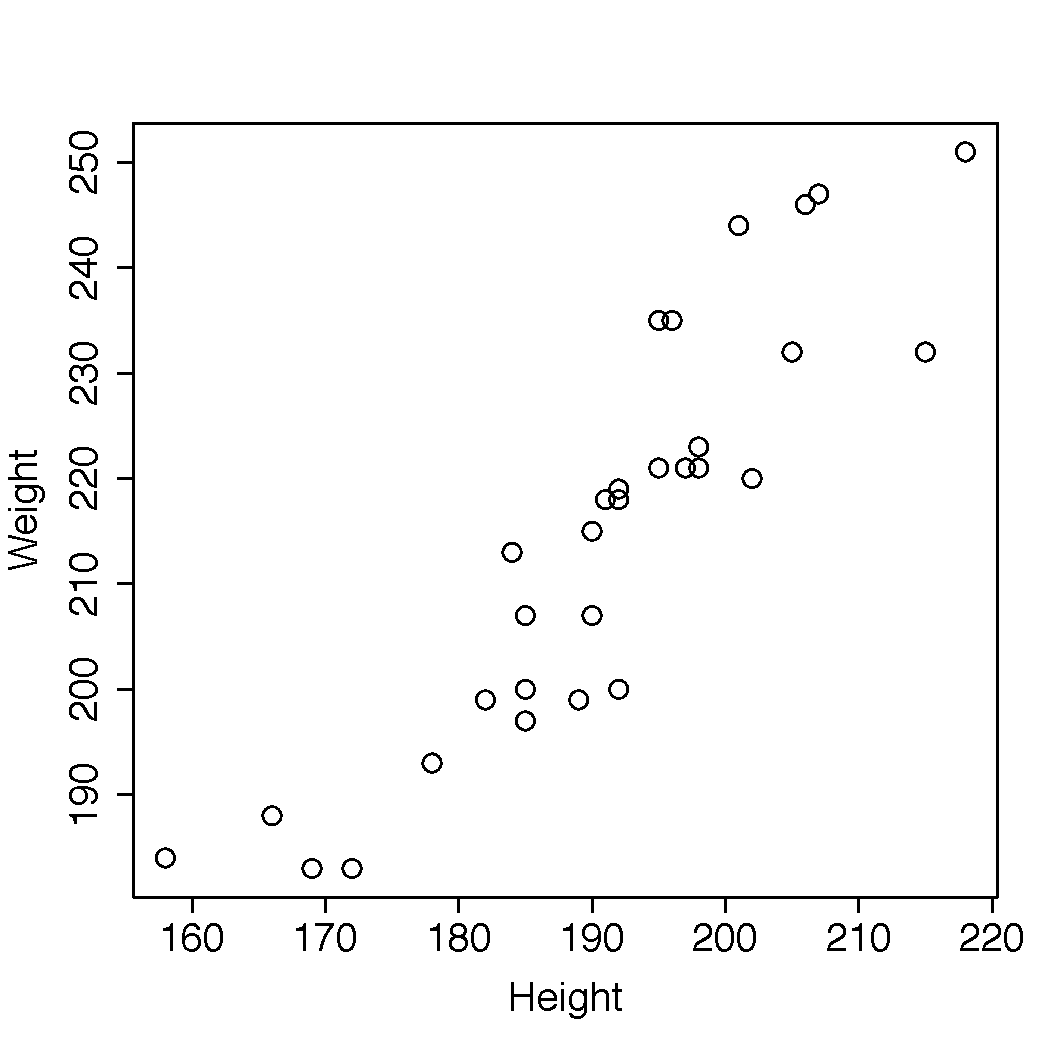
\includegraphics[width=0.58\textwidth]{images/DataEx-Basketball_Scatter_Height_Weight.pdf}
\caption{An example scatter plot showing the relationship between the \featN{Height} and \featN{Weight} features from the professional basketball squad dataset in Table \ourRef{table:proBasketballTeamDataset}.}
\label{fig:scatterPlotExample}

\end{figure}
\end{frame} 



 \begin{frame} 
\begin{figure}[!htb]
\subfigure[]{\label{fig:scatterPlotsVarNegCorr}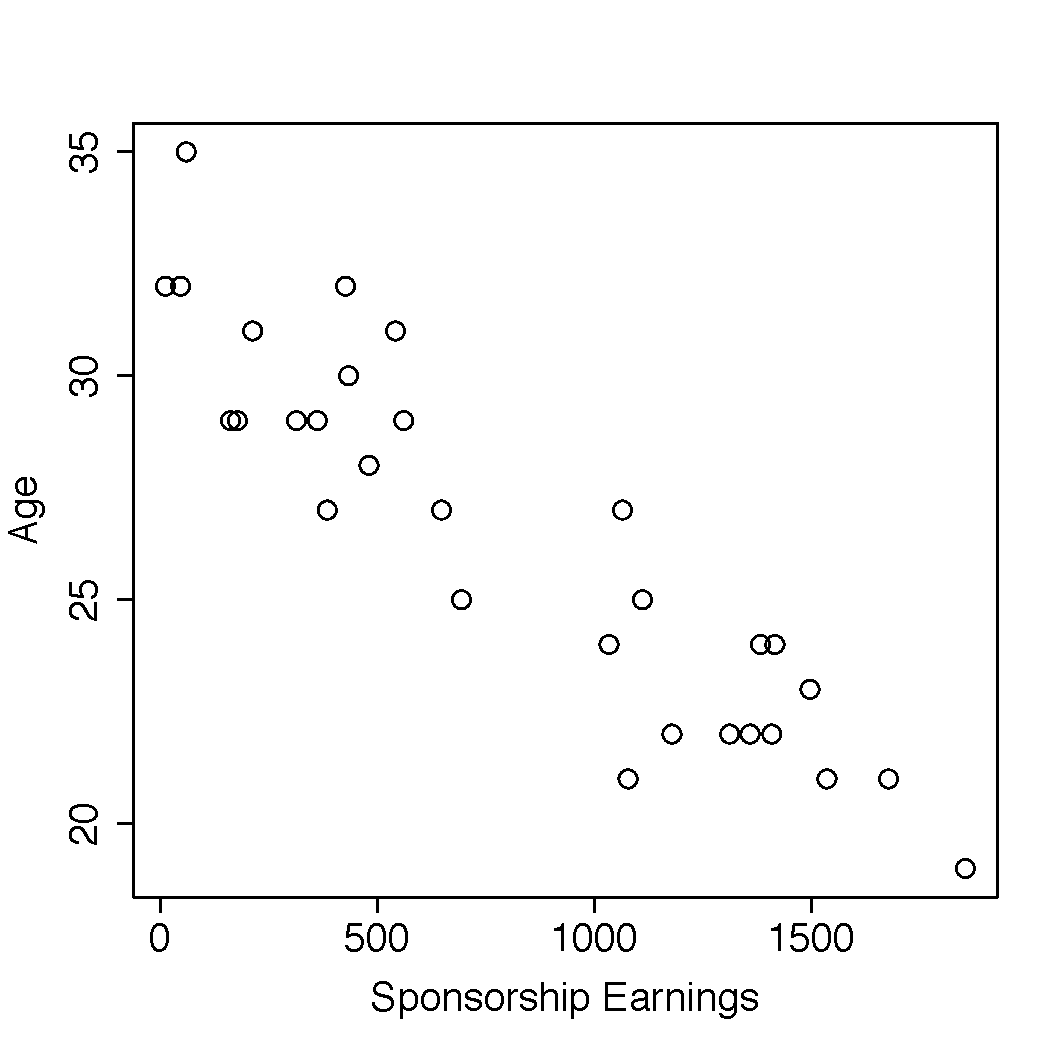
\includegraphics[width=0.48\textwidth]{images/DataEx-Basketball_Scatter_Sponsorship_Age.pdf}}
\subfigure[]{\label{fig:scatterPlotsVarNoCorr}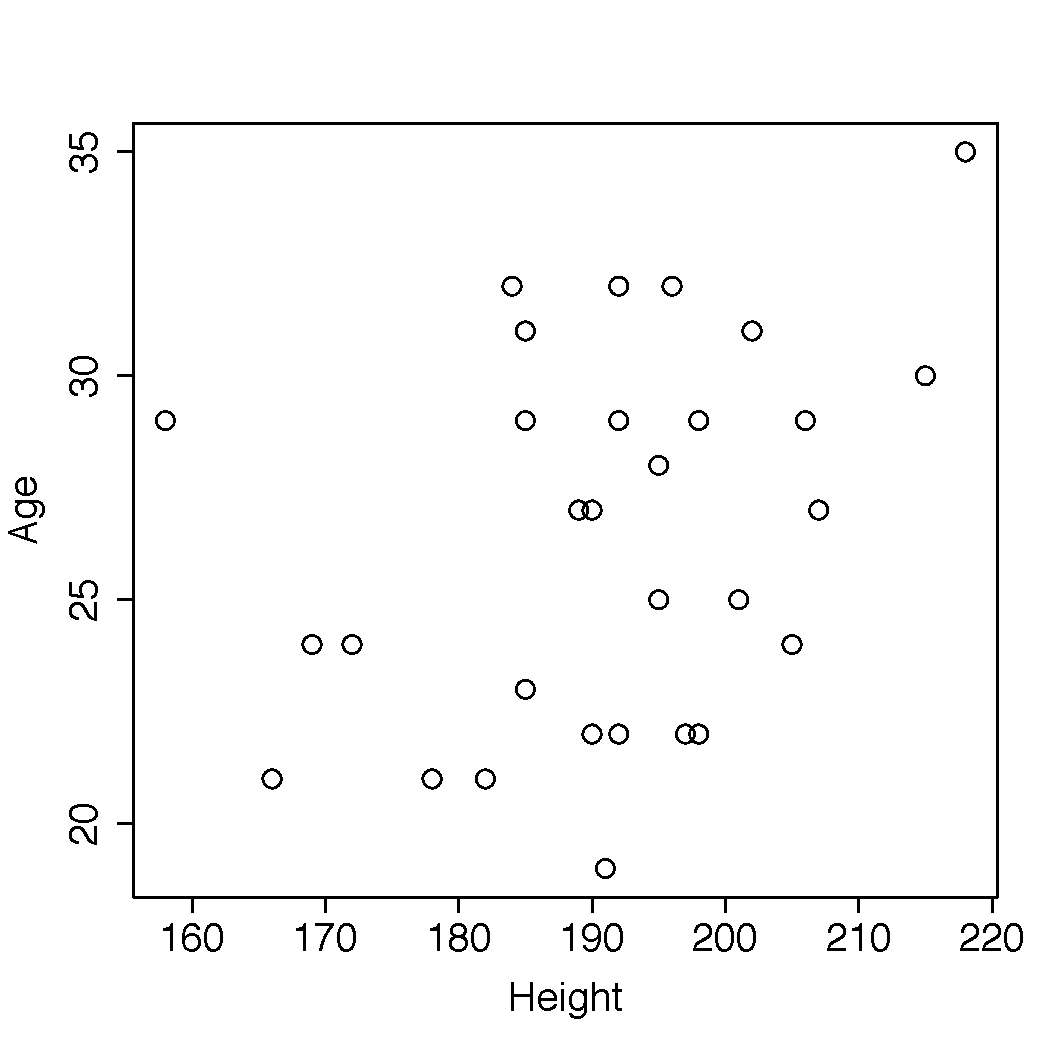
\includegraphics[width=0.48\textwidth]{images/DataEx-Basketball_Scatter_Height_Age.pdf}} 
\caption{Example scatter plots showing (a) the strong negative covariance between the \featN{Sponsorship Earnings} and \featN{Age} features and (b) the \featN{Height} and \featN{Age} features from the dataset in Table \ourRef{table:proBasketballTeamDataset}.}
\label{fig:scatterPlotsVar}
\end{figure}
\end{frame} 

\begin{frame}
	\begin{itemize}
		\item A \indexkeyword{scatter plot matrix} (\indexkeyword{SPLOM}) shows scatter plots for a whole collection of features arranged into a matrix. 
		\item This is useful for exploring the relationships between groups of features - for example all of the continuous features in an ABT.
	\end{itemize}
\end{frame}


\begin{frame} [plain]
	\begin{figure}
	\centering
	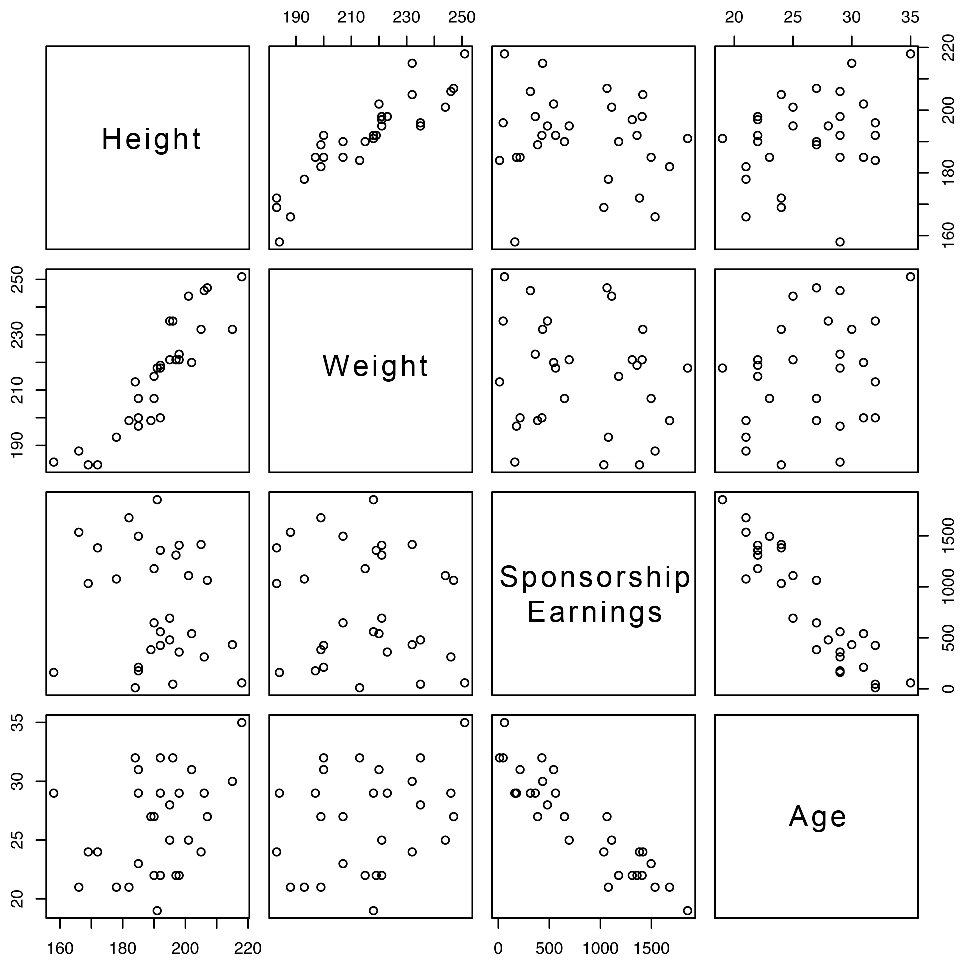
\includegraphics[width=0.75\textwidth]{images/DataEx-Basketball_SPLOM_Mod.pdf}
	\caption{A scatter plot matrix showing scatter plots of the continuous features from the professional basketball squad dataset.}
	\label{fig:scatterPlotMatrixExample}
	\end{figure}
\end{frame} 


\begin{frame}
	\begin{itemize}
		\item The simplest way to visualize the relationship between two categorical variables is to use a collection of \keyword{small multiple} bar plots.
	\end{itemize}
\end{frame}


 \begin{frame} 
\begin{figure}
\centering
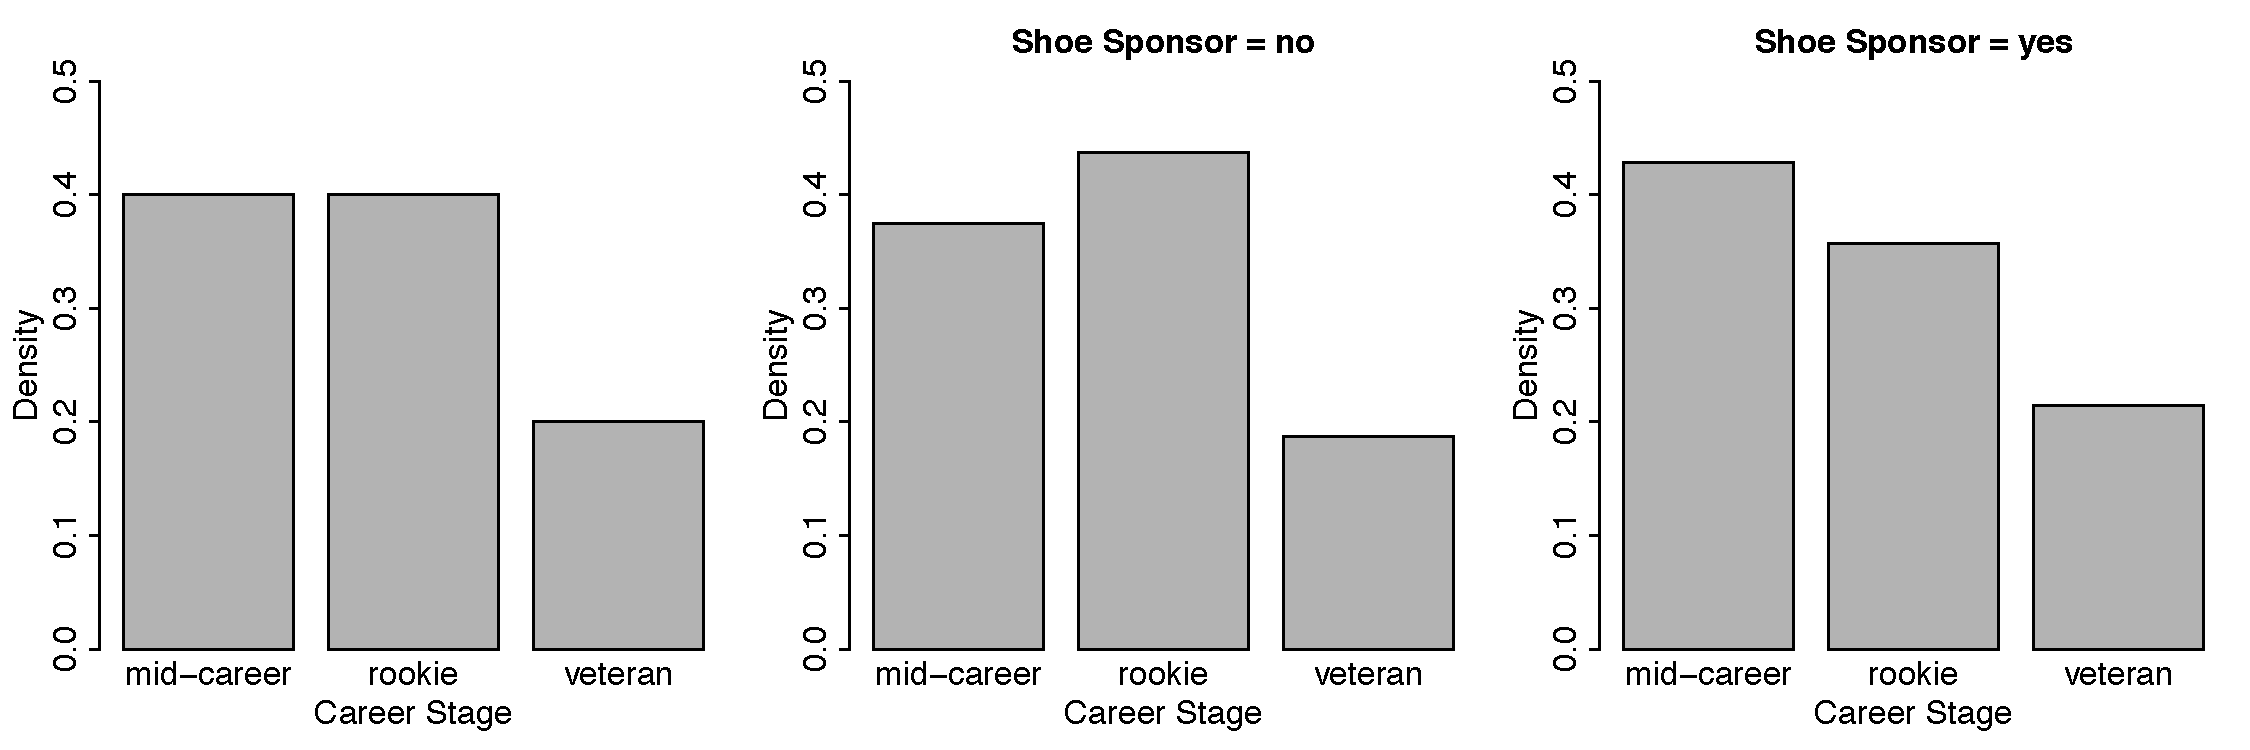
\includegraphics[width=0.99\textwidth]{images/DataEx-Basketball_SmallMulBarPlot_Shoes_CareerStage.pdf}
\caption{Using small multiple bar plot visualizations to illustrate the relationship between the \featN{Career Stage} and \featN{Shoe Sponsor} features.}
\label{fig:barPlotSmallMultipleExample1}
\end{figure}
\end{frame} 

 \begin{frame} 
\begin{figure}
\centering
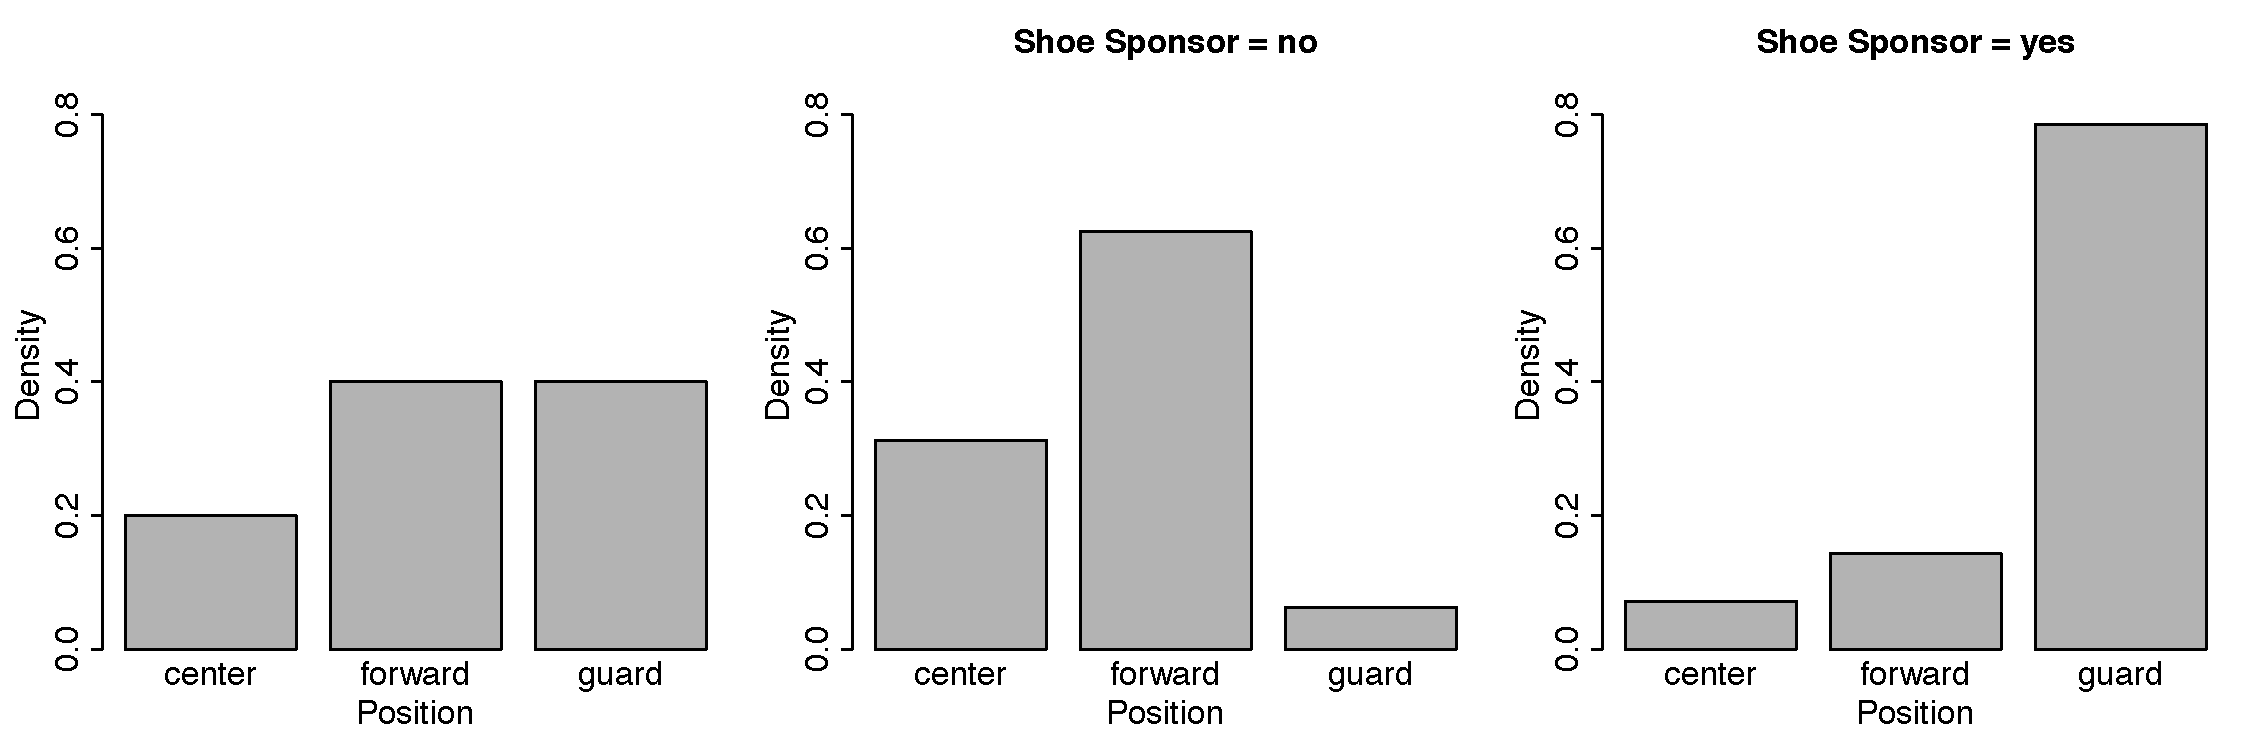
\includegraphics[width=0.99\textwidth]{images/DataEx-Basketball_SmallMulBarPlot_Shoes_Position.pdf}
\caption{Using small multiple bar plot visualizations to illustrate the relationship between the \featN{Position} and \featN{Shoe Sponsor} features.}
\label{fig:barPlotSmallMultipleExample2}
\end{figure}
\end{frame} 




\begin{frame}
	\begin{itemize}
		\item If the number of levels of one of the features being compared is no more than three we can use \keyword{stacked bar plots} as an alternative to the small multiples approach. 
	\end{itemize}
\end{frame}


 \begin{frame}[plain] 
\begin{figure}
\centering
\subfigure[Career Stage and Shoe Sponsor]{\label{fig:stackedBarPlotExample1}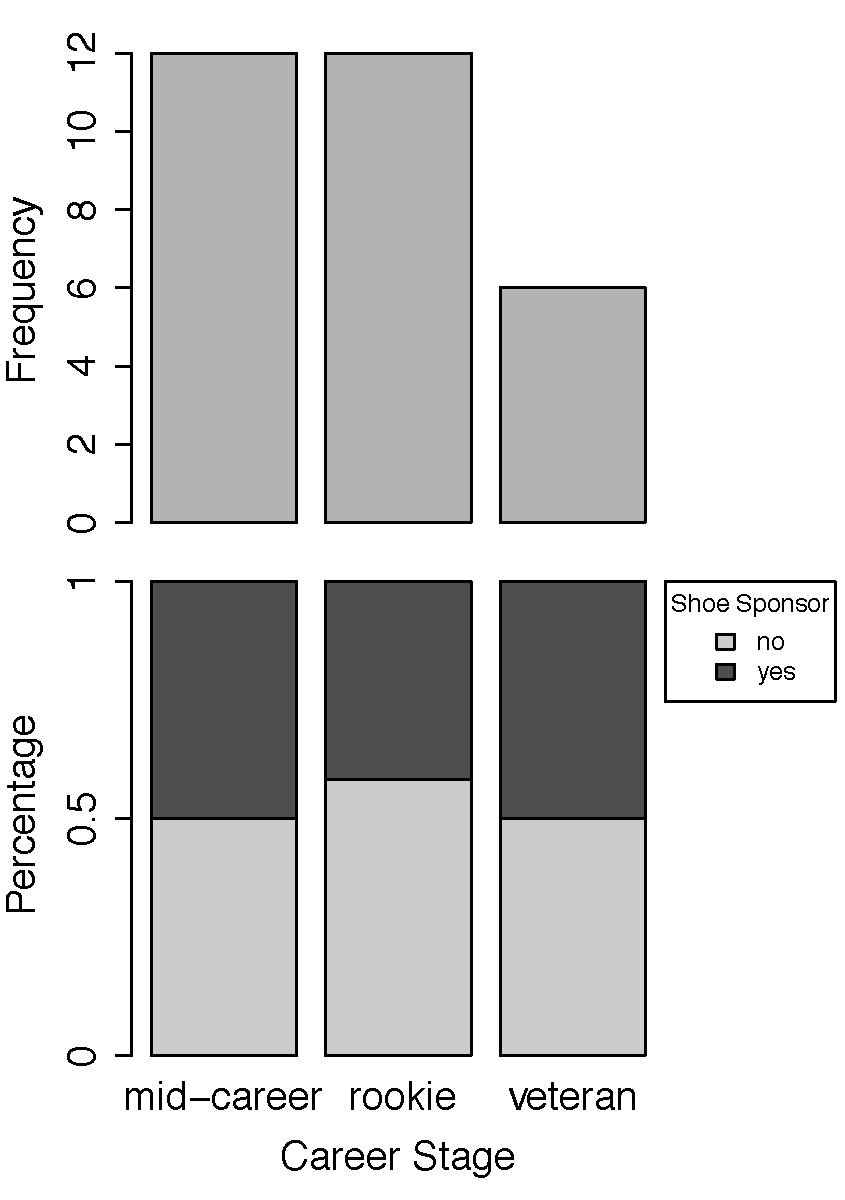
\includegraphics[width=0.44\textwidth]{images/DataEx-Basketball_StackedBarPlot_Shoes_CareerStage}}
\subfigure[Position and Shoe Sponsor]{\label{fig:stackedBarPlotExample2}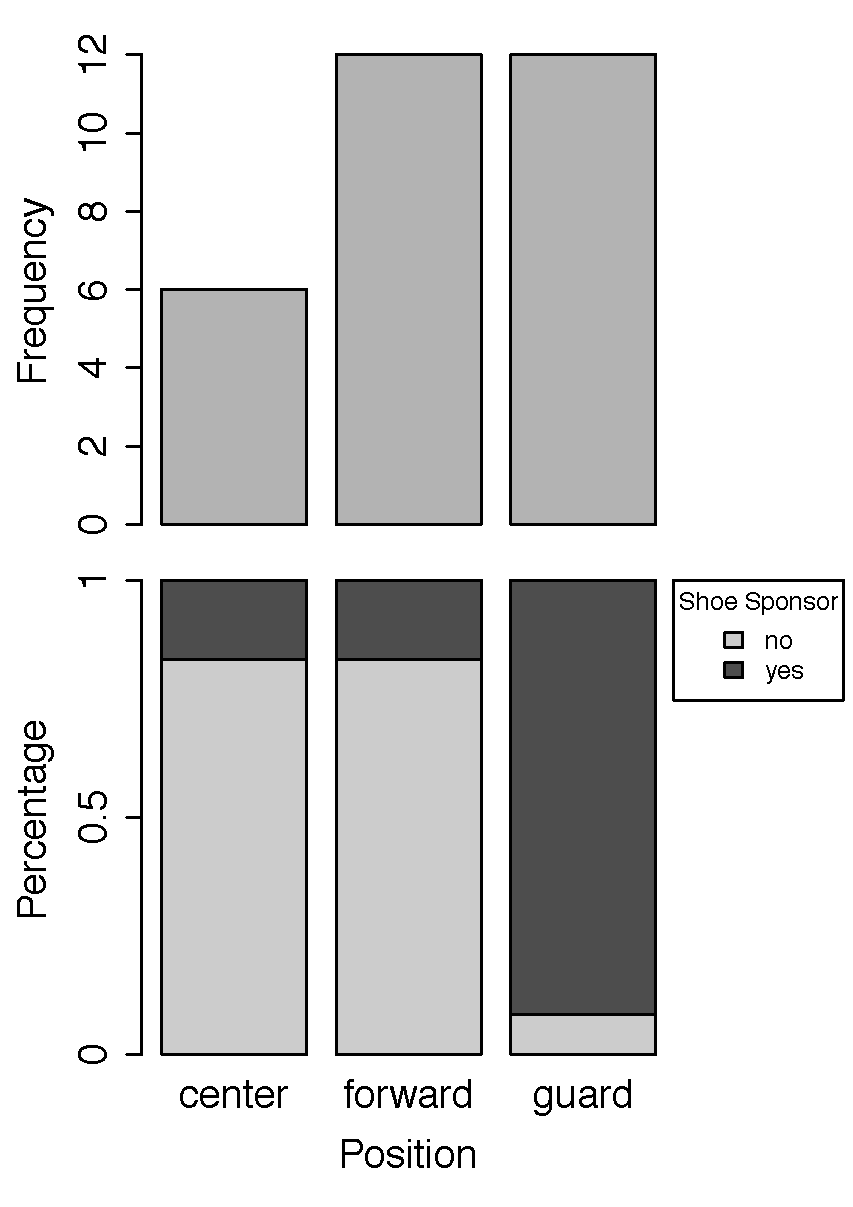
\includegraphics[width=0.44\textwidth]{images/DataEx-Basketball_StackedBarPlot_Shoes_Position.pdf}}
\caption{Stacked bar plot visualizations.}
\label{fig:stackedBarPlotExample}

\end{figure}
\end{frame} 


\begin{frame}
	\begin{itemize}
		\item To visualize  the relationship between a continuous feature and a categorical feature a \indexkeyword{small multiples} approach that draws a histogram of the values of the continuous feature for each level of the categorical feature is useful. 
	\end{itemize}
\end{frame}

 \begin{frame}  [plain]
\begin{figure}
\centering
\subfigure[Age]{\label{fig:histogramSmallMultipleExampleAgeFull}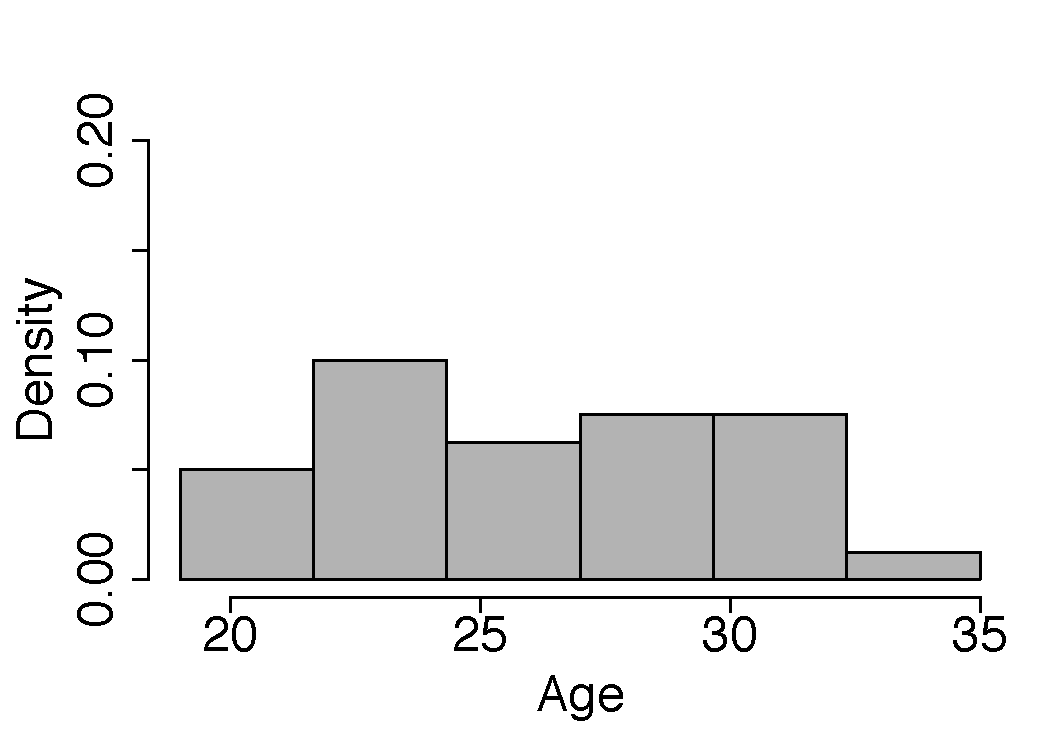
\includegraphics[width=0.35\textwidth]{images/DataEx-BasketballHist_Age.pdf}}
\subfigure[Age and Position]{\label{fig:histogramSmallMultipleExampleAgePosition}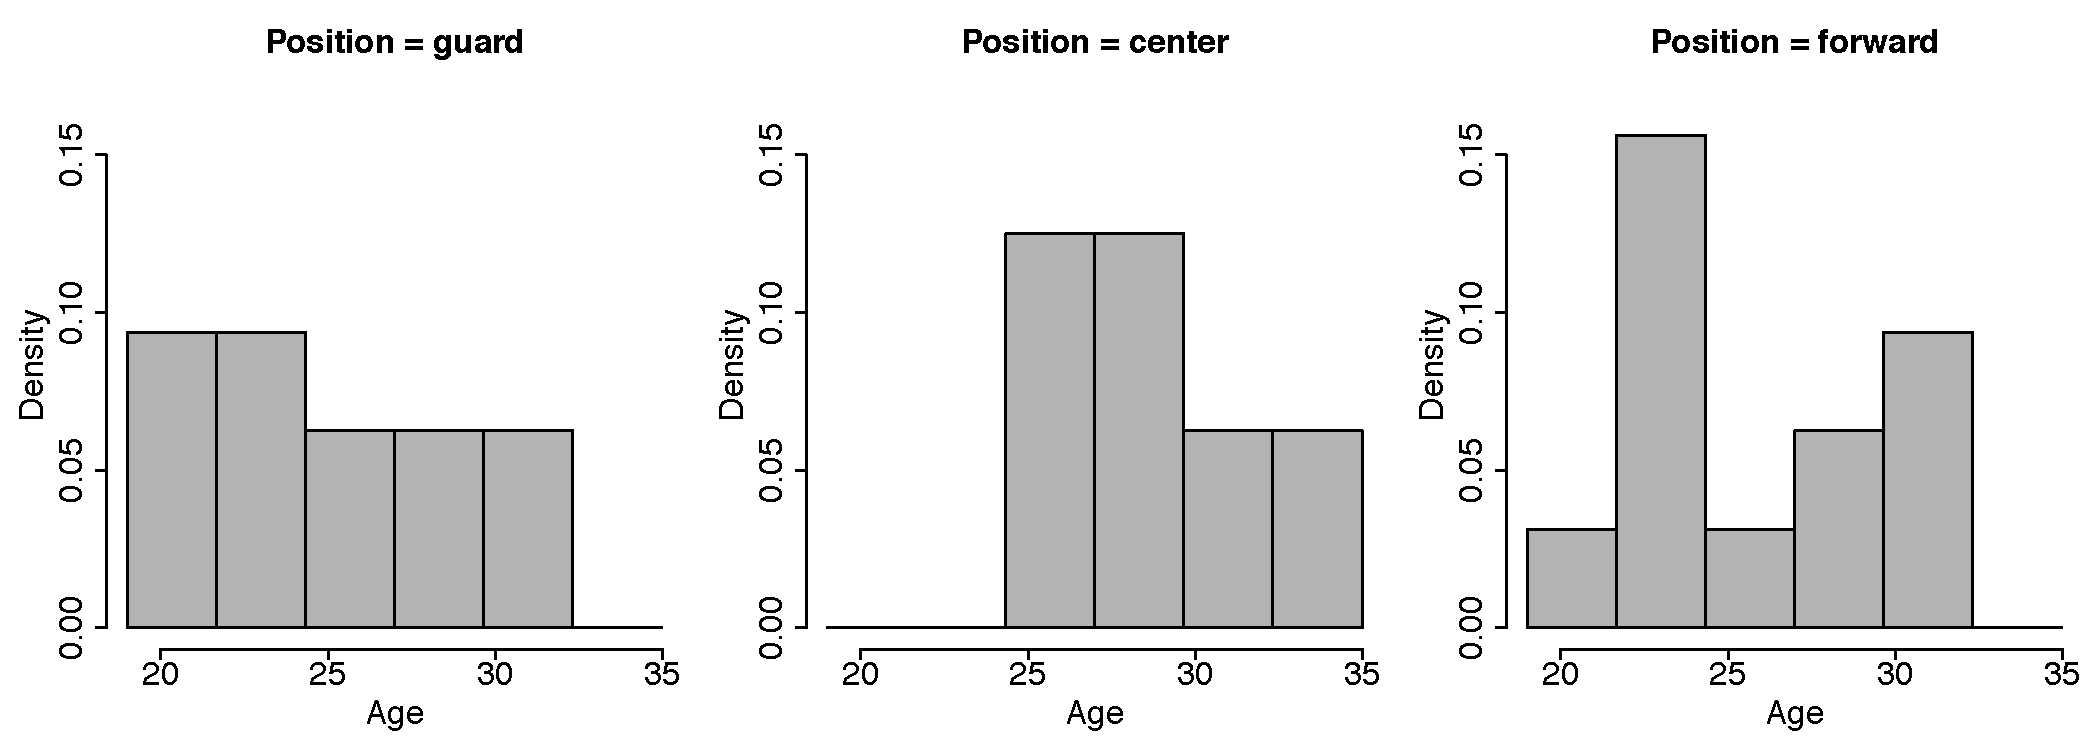
\includegraphics[width=0.93\textwidth]{images/DataEx-BasketballHist_Age_Position.pdf}}
\caption{Using small multiple histograms to visualize the relationship between the \featN{Age} feature and the \featN{Position feature}.}
\label{fig:histogramSmallMultipleExample1}
\end{figure}
\end{frame} 

 \begin{frame} [plain]
\begin{figure}
\centering
\subfigure[Height]{\label{fig:histogramSmallMultipleExampleHeightFull}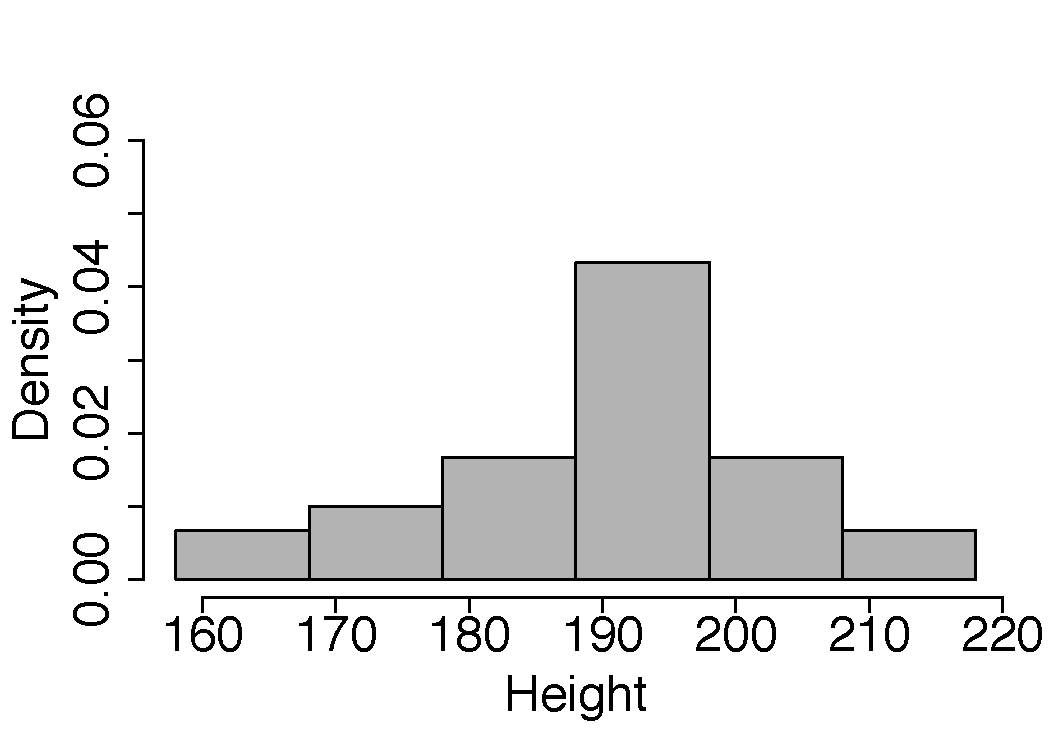
\includegraphics[width=0.35\textwidth]{images/DataEx-BasketballHistHeight.pdf}}
\subfigure[Height and Position]{\label{fig:histogramSmallMultipleExampleHeightPosition}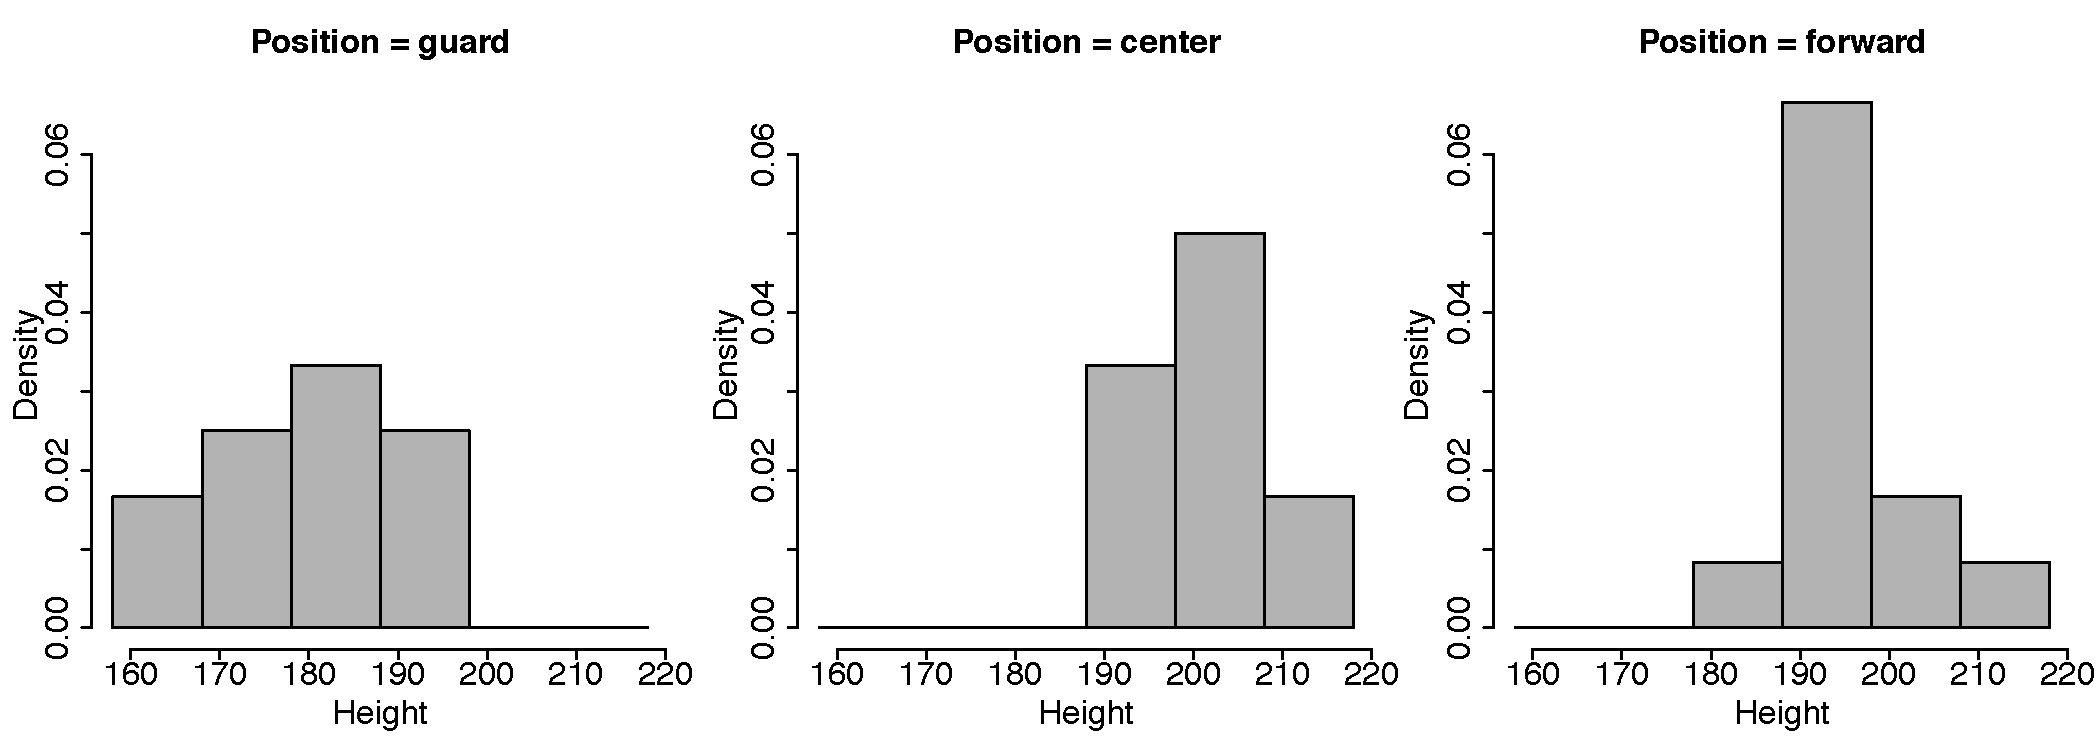
\includegraphics[width=0.93\textwidth]{images/DataEx-BasketballHist_Height_Position.pdf}}
\caption{Using small multiple histograms to visualize the relationship between the \featN{Height} feature and the \featN{Position} feature.}
\label{fig:histogramSmallMultipleExample2}

\end{figure}
\end{frame} 


\begin{frame}
	\begin{itemize}
		\item A second approach to visualizing the relationship between a categorical feature and a continuous feature is to use a collection of box plots. 
		\item For each level of the categorical feature a box plot of the corresponding values of the continuous feature is drawn. 
	\end{itemize}
\end{frame}


 \begin{frame} [plain]
\begin{figure}
\centering
\subfigure[Age]{\label{fig:boxPlotPlotExampleAge}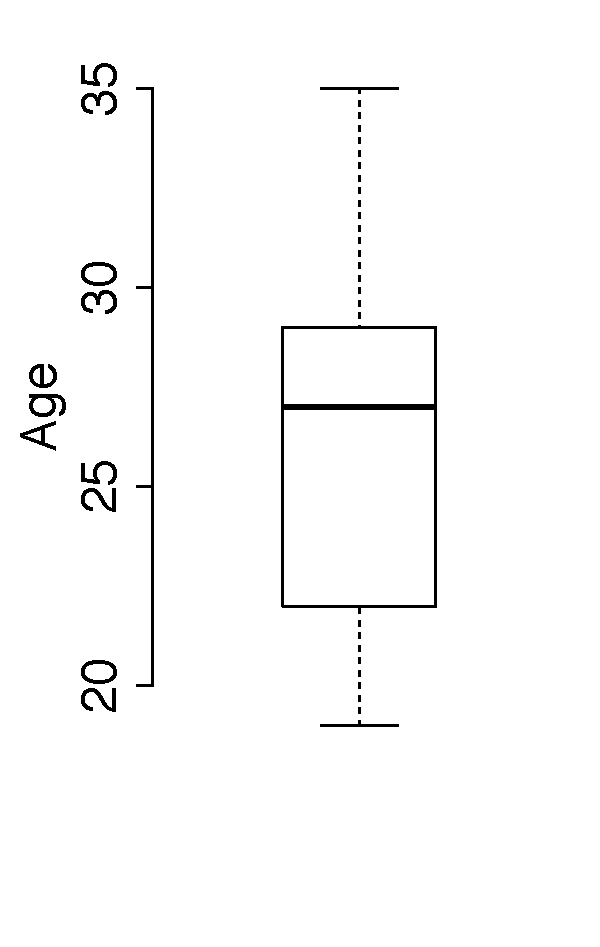
\includegraphics[width=0.3\textwidth]{images/DataEx-BasketballBoxPlot_Age.pdf}}
\subfigure[Age and Position]{\label{fig:boxPlotPlotExampleAgePosition}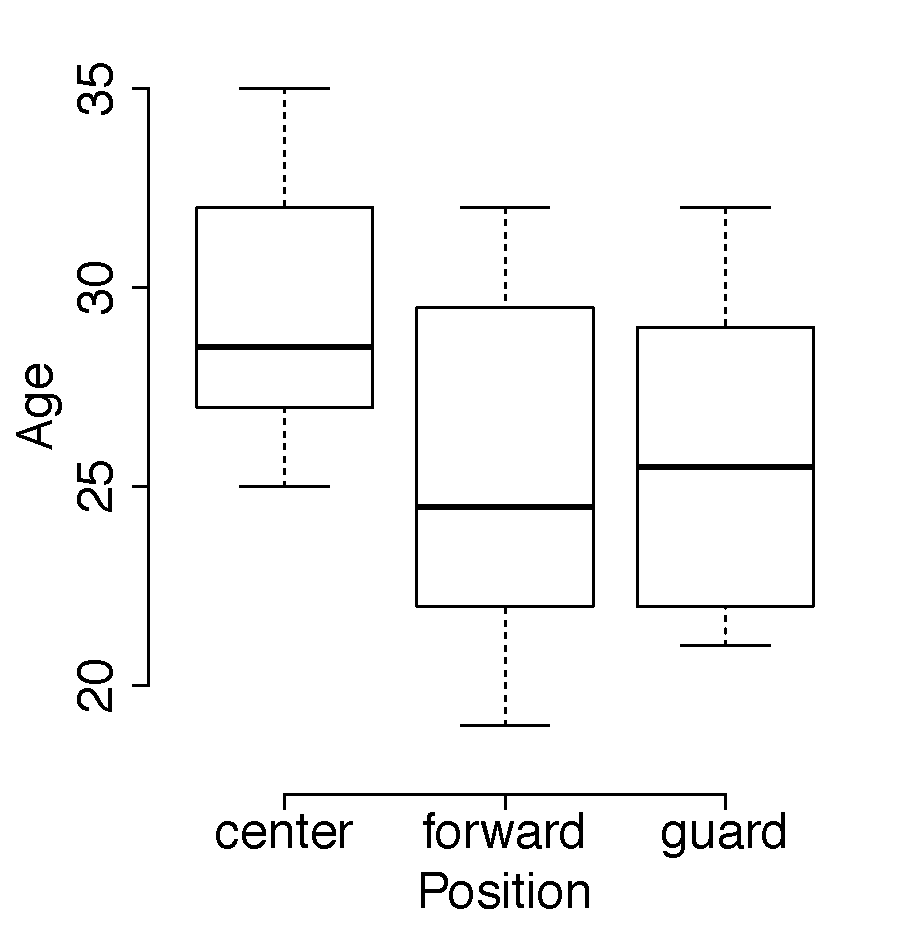
\includegraphics[width=0.45\textwidth]{images/DataEx-BasketballBoxPlot_Age_Position.pdf}}
\caption{Using box plots to visualize the relationship between the \featN{Age} and the \featN{Position} feature.}
\label{fig:boxPlotPlotExample}

\end{figure}
\end{frame} 

 \begin{frame} [plain]
\begin{figure}
\centering
\subfigure[Height]{\label{fig:boxPlotPlotExampleHeight}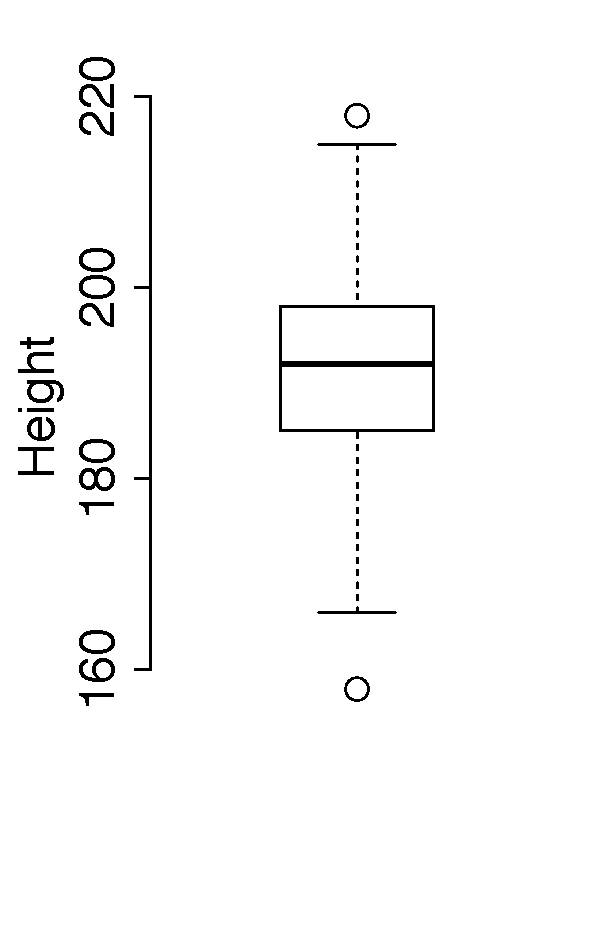
\includegraphics[width=0.3\textwidth]{images/DataEx-BasketballBoxPlot_Height.pdf}}
\subfigure[Height and Position]{\label{fig:boxPlotPlotExampleHeightPosition}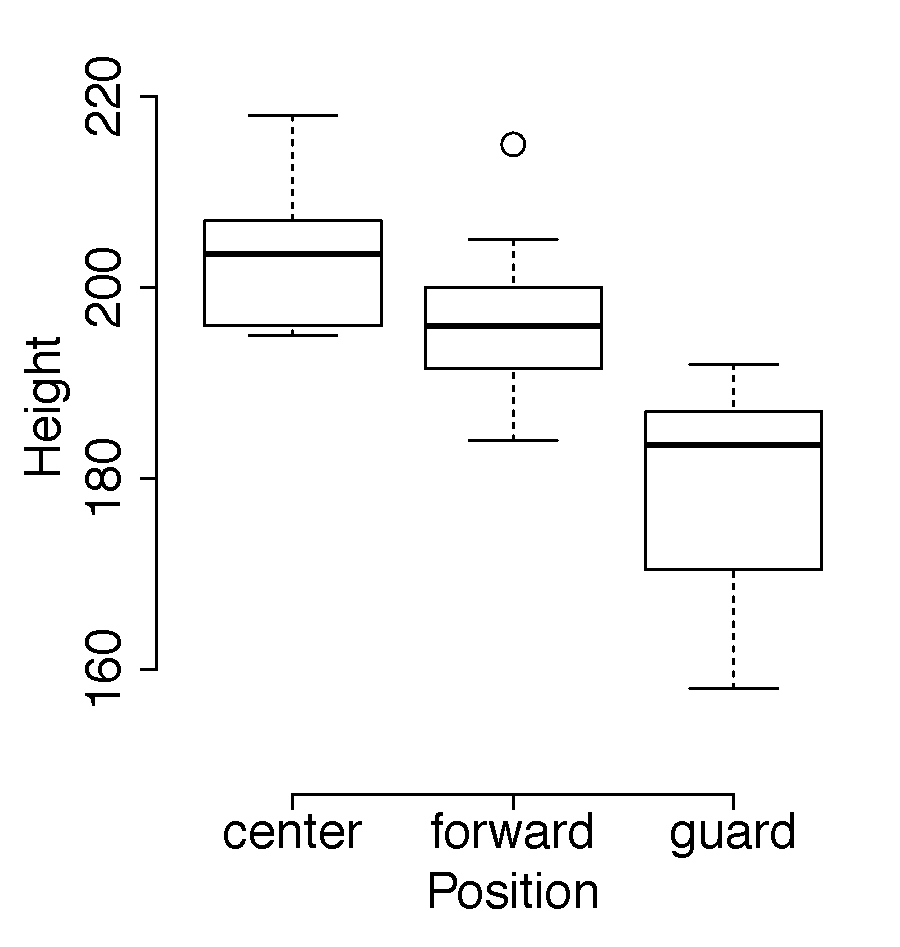
\includegraphics[width=0.45\textwidth]{images/DataEx-BasketballBoxPlot_Height_Position.pdf}}
\caption{Using box plots to visualize the relationship between the \featN{Height} feature and the \featN{Position} feature. }
\label{fig:boxPlotPlotExample}

\end{figure}
\end{frame} 


\subsection{Measuring Covariance \& Correlation}

 \begin{frame} 
 \begin{itemize}
		\item As well as visually inspecting scatter plots, we can calculate formal measures of the relationship between two continuous features using \keyword{covariance} and \keyword{correlation}. 
		\item For two features, $a$ and $b$, in a dataset of $n$ instances, the \keyword{sample covariance} between $a$ and $b$ is
\begin{equation}
cov(a,b)=\frac{1}{n - 1}\displaystyle \sum_{i=1}^{n} \left( \left( a_i - \overline{a} \right) \times \left(b_i - \overline{b} \right)\right)
\label{eq:cov}
\end{equation}
\noindent where $a_i$ and $b_i$ are values of features $a$ and $b$ for the $i^{th}$ instance in a dataset, and $\overline{a}$ and $\overline{b}$ are the sample means of features $a$ and $b$. 
	\end{itemize}

\end{frame} 

 \begin{frame} 
 \begin{itemize}
		\item Covariance values fall into the range $[-\infty, \infty]$ where negative values indicate a negative relationship, positive values indicate a positive relationship, and values near zero indicate that there is little or no relationship between the features.
	\end{itemize}

\end{frame} 


 \begin{frame} [plain]
Calculating covariance between  the \featN{Height} feature and the \featN{Weight} and \featN{Age} features from the basketball players dataset. 
\begin{overprint}
\onslide<1>
\begin{table}[htb]
\label{table:covarExample}
\centering
\begin{footnotesize}
\resizebox{\textwidth}{!}{\begin{tabular}{  r c r c r r c r r}
\hline
	~	&	\featN{Height}	&	~ &	\featN{Weight}	&	~	&	$(h - \overline{h})\times$	&	\featN{Age}	&	~&	$(h - \overline{h})\times$ 	\\
	\featN{ID}	&	($h$)	&	$h - \overline{h}$ &	($w$)	&	$w - \overline{w}$	&	$(w - \overline{w})$	&	($a$)	&	$a - \overline{a}$	&	$(a - \overline{a})$	\\
\hline	
1	&	192	&	0.9	&	218	&	3.0	&	2.7	&	29	&	2.6	&	2.3	\\
2	&	218	&	26.9	&	251	&	36.0	&	967.5	&	35	&	8.6	&	231.3	\\
3	&	197	&	5.9	&	221	&	6.0	&	35.2	&	22	&	-4.4	&	-26.0	\\
4	&	192	&	0.9	&	219	&	4.0	&	3.6	&	22	&	-4.4	&	-4.0	\\
5	&	198	&	6.9	&	223	&	8.0	&	55.0	&	29	&	2.6	&	17.9	\\
\multicolumn{9}{c}{$\dots$} \\
26	&	191	&	-0.1	&	218	&	3.0	&	-0.3	&	19	&	-7.4	&	0.7	\\
27	&	196	&	4.9	&	235	&	20.0	&	97.8	&	32	&	5.6	&	27.4	\\
28	&	198	&	6.9	&	221	&	6.0	&	41.2	&	22	&	-4.4	&	-30.4	\\
29	&	207	&	15.9	&	247	&	32.0	&	508.3	&	27	&	0.6	&	9.5	\\
30	&	201	&	9.9	&	244	&	29.0	&	286.8	&	25	&	-1.4	&	-13.9	\\
\hline
\textbf{Mean}	&	191.1	&		&	215.0	&		&		&	26.4	&		&		\\
\textbf{Std Dev}	&	13.6	&		&	19.8	&		&		&	4.2	&		&		\\
\textbf{Sum}	&		&		&		&		&	7,009.9	&		&		&	570.8	\\
\hline
\end{tabular}}
\end{footnotesize}
\end{table}
\onslide<2>
\begin{alignat*}{5}
cov(\featN{Height},\featN{Weight}) & = &\;\frac{7{,}009.9}{29} & = & \;241.72  \\
cov(\featN{Height},\featN{Age}) & = & \frac{570.8}{29} & = & 19.7 
\end{alignat*}
\end{overprint}
\end{frame} 





 \begin{frame} 
  \begin{itemize}
		\item \keyword{Correlation} is a normalized form of covariance that ranges between $-1$ and $+1$.  
		\item The correlation between two features, $a$ and $b$, can be calculated as
\begin{alignat}{2}
corr(a,b) & = \frac{cov(a, b)}{sd(a) \times sd(b)} % \\
\label{eq:corr}
\end{alignat}
\noindent where $cov(a, b)$ is the covariance between features $a$ and $b$ and $sd(a)$ and $sd(b)$ are the standard deviations of $a$ and $b$ respectively.  
	\end{itemize}
\end{frame} 

 \begin{frame} 
  \begin{itemize}
		\item Correlation values fall  into the range $\left[-1, 1\right]$, where values close to $-1$ indicate a very strong negative correlation (or covariance), values close to $1$ indicate a very strong positive correlation, and values around $0$ indicate no correlation. 
		\item Features that have no correlation are said to be \keyword{independent}. 
	\end{itemize}
\end{frame} 

 \begin{frame} 
 Calculating correlation between  the \featN{Height} feature and the \featN{Weight} and \featN{Age} features from the basketball players dataset. 
\begin{alignat*}{3}
corr(Height,Weight) & = \frac{241.72}{13.6 \times 19.8}\; & = 0.898 \\
corr(Height,Age) & = \frac{19.7}{13.6 \times 4.2}\; & = 0.345
\label{eq:corrExamples}
\end{alignat*}
\end{frame} 



 \begin{frame} 
  \begin{itemize}
		\item In the majority of ABTs there are multiple continuous features between which we would like to explore relationships. 
		\item Two tools that can be useful for this are the covariance matrix and the correlation matrix. 
\end{itemize}
\end{frame} 

 \begin{frame} 
  \begin{itemize}
		\item The covariance matrix, usually denoted as $\sum$, between a set of continuous features, $\{a, b, \ldots, z\}$, is given as
		\end{itemize}
\begin{equation}
\sum_{\{a,b,\ldots,z\}}=
\begin{bmatrix}
var(a) & cov(a,b) & \cdots &cov(a,z) \\
cov(b,a) & var(b) & \cdots & cov(b,z) \\
\vdots & \vdots & \ddots & \vdots \\
cov(z,a) & cov(z,b) & \cdots & var(z) 
\end{bmatrix}
\label{eq:covMatrix}
\end{equation}
\end{frame} 

 \begin{frame} 
  \begin{itemize}
\item Similarly, the \indexkeyword{correlation matrix} is just a normalized version of the covariance matrix and shows the correlation between each pair of features:
\end{itemize}
\begin{equation}
\underset{\{a,b,\ldots,z\}}{correlation~matrix} = 
\begin{bmatrix}
corr(a, a) & corr(a,b) & \cdots &corr(a,z) \\
corr(b,a) & corr(b, b) & \cdots & corr(b,z) \\
\vdots & \vdots & \ddots & \vdots \\
corr(z,a) & corr(z,b) & \cdots & corr(z, z) 
\end{bmatrix}
\label{eq:corrMatrix}
\end{equation}
\end{frame} 



 \begin{frame} 
\begin{itemize}
\item Calculating covariances matrix for the \featN{Height} feature and the \featN{Weight} and \featN{Age} features from the basketball players dataset. 
\end{itemize}
\begin{equation*}
\sum_{<Height, Weight, Age>}=
\begin{bmatrix}
185.128	& 241.72 & 19.7 \\
241.72	& 392.102 & 24.469 \\
19.7	& 24.469 & 17.697 
\end{bmatrix}
\label{eq:covmatrixexample}
\end{equation*}
\end{frame} 



 \begin{frame} 
\begin{itemize}
\item Calculating correlation matrix for the \featN{Height} feature and the \featN{Weight} and \featN{Age} features from the basketball players dataset.  
\end{itemize}
\begin{equation*}
\underset{<Height, Weight, Age>}{\text{correlation matrix}} =
\begin{bmatrix}
1.0	& 0.898	& 0.345 \\
0.898	& 1.0	& 0.294 \\
0.345 & 0.294	& 1.0 \\
\end{bmatrix}
\label{eq:covmatrix}
\end{equation*}
\end{frame} 


 \begin{frame} 
\begin{itemize}
\item The \keyword{scatter plot matrix} (SPLOM) is really a visualization of the correlation matrix. 
\item This can be made more obvious by including the correlation coefficients in SPLOMs in the cells above the diagonal. 
\end{itemize}
\end{frame} 


 \begin{frame} [plain]
\begin{figure}
\centering
\includegraphics[width=0.85\textwidth]{images/DataEx-Basketball_SPLOM_Fancy_Adjusted_mod_2.pdf}
\end{figure}
\end{frame} 



 \begin{frame} 
\begin{itemize}
\item Correlation is a good measure of the relationship between two continuous features, but it is not by any means perfect.
\item Some of the limitations of measuring correlation are illustrated very clearly in the famous example of \indexkeyword{Anscombe's quartet} by \keyword{Francis Anscombe}.
\end{itemize}
\end{frame} 

 \begin{frame} [plain]
\begin{figure}
\centering
\subfigure{\label{fig:anscombesQuartet1}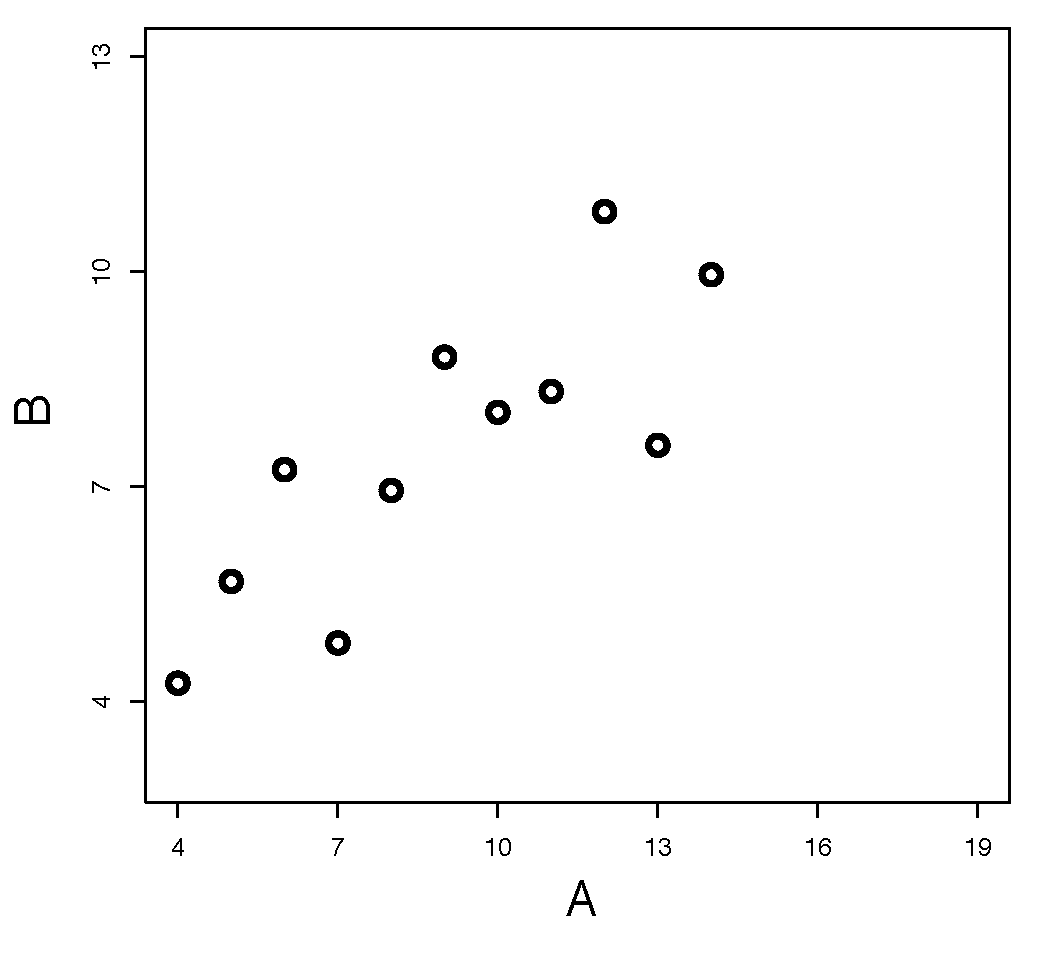
\includegraphics[width=0.4\textwidth]{images/DataEx-Anscombe1.pdf}}
\subfigure{\label{fig:anscombesQuartet2}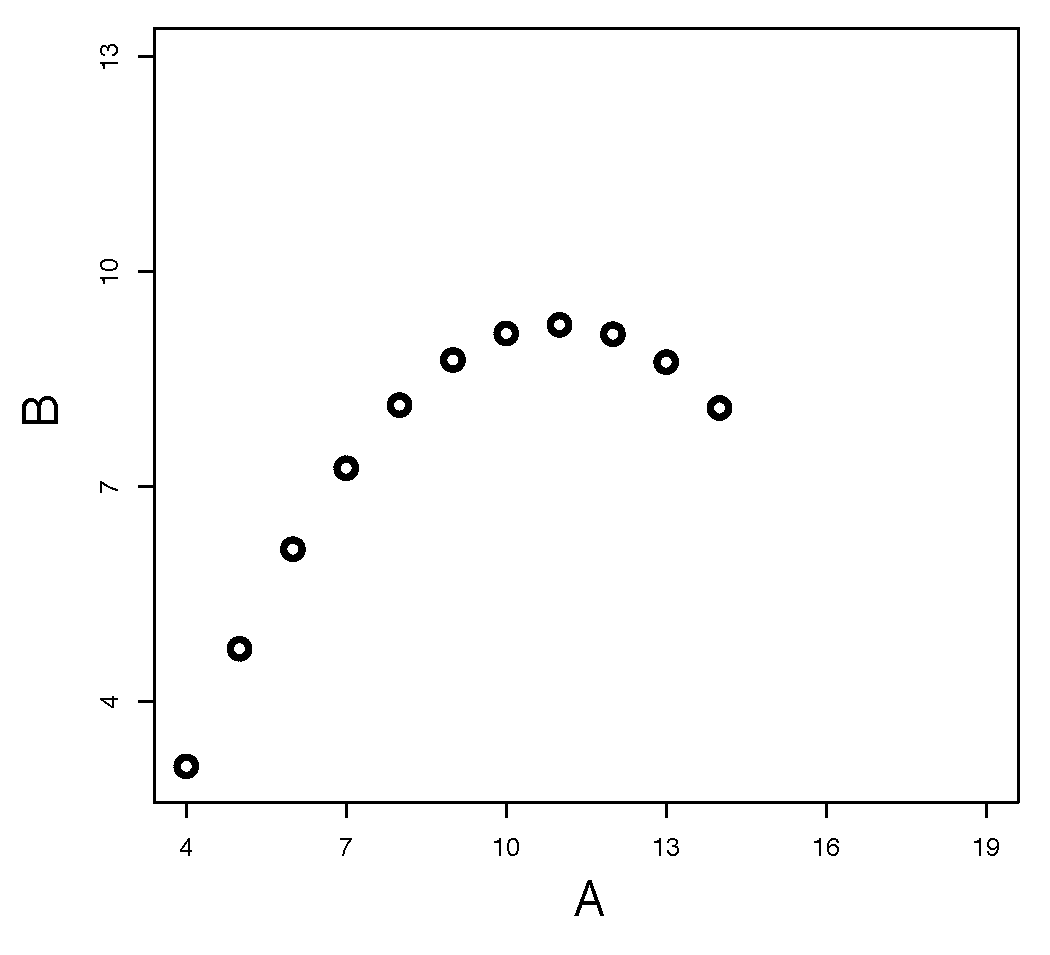
\includegraphics[width=0.4\textwidth]{images/DataEx-Anscombe2.pdf}}  \\
\subfigure{\label{fig:anscombesQuartet3}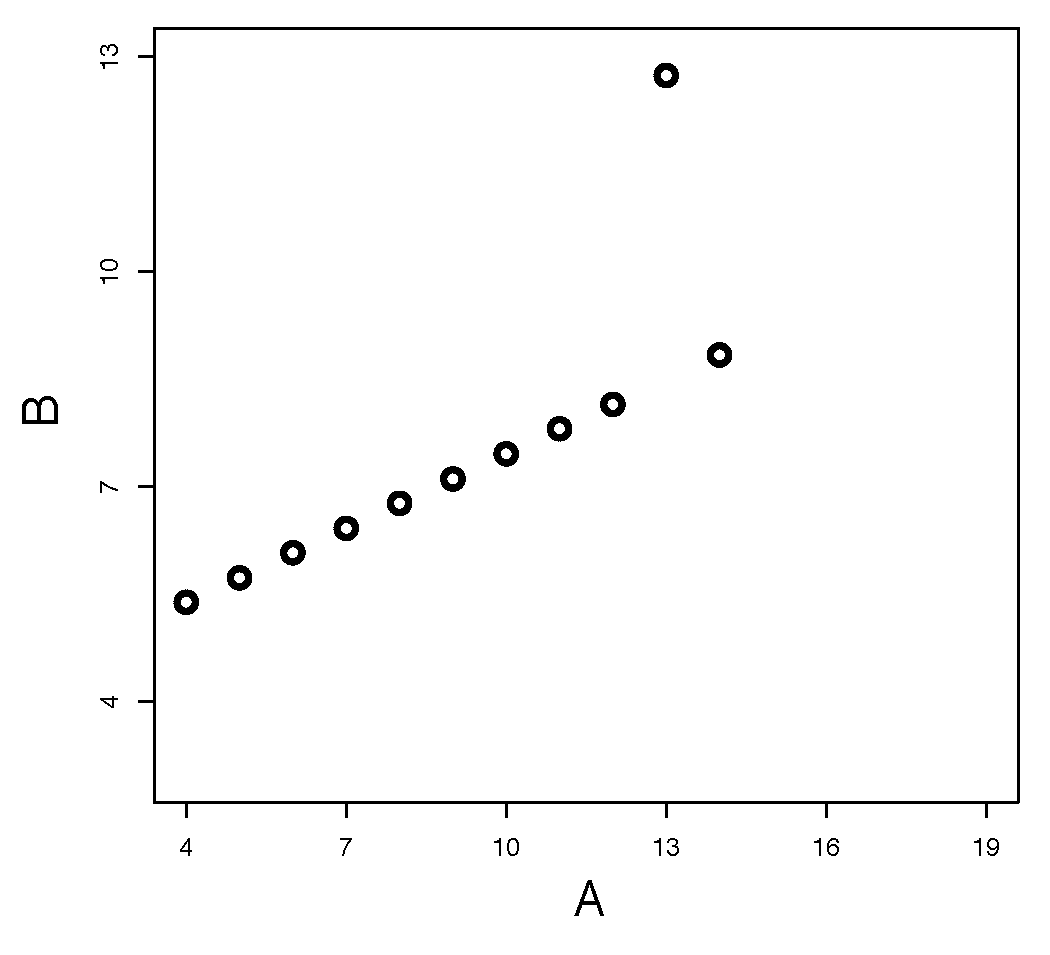
\includegraphics[width=0.4\textwidth]{images/DataEx-Anscombe3.pdf}}
\subfigure{\label{fig:anscombesQuartet4}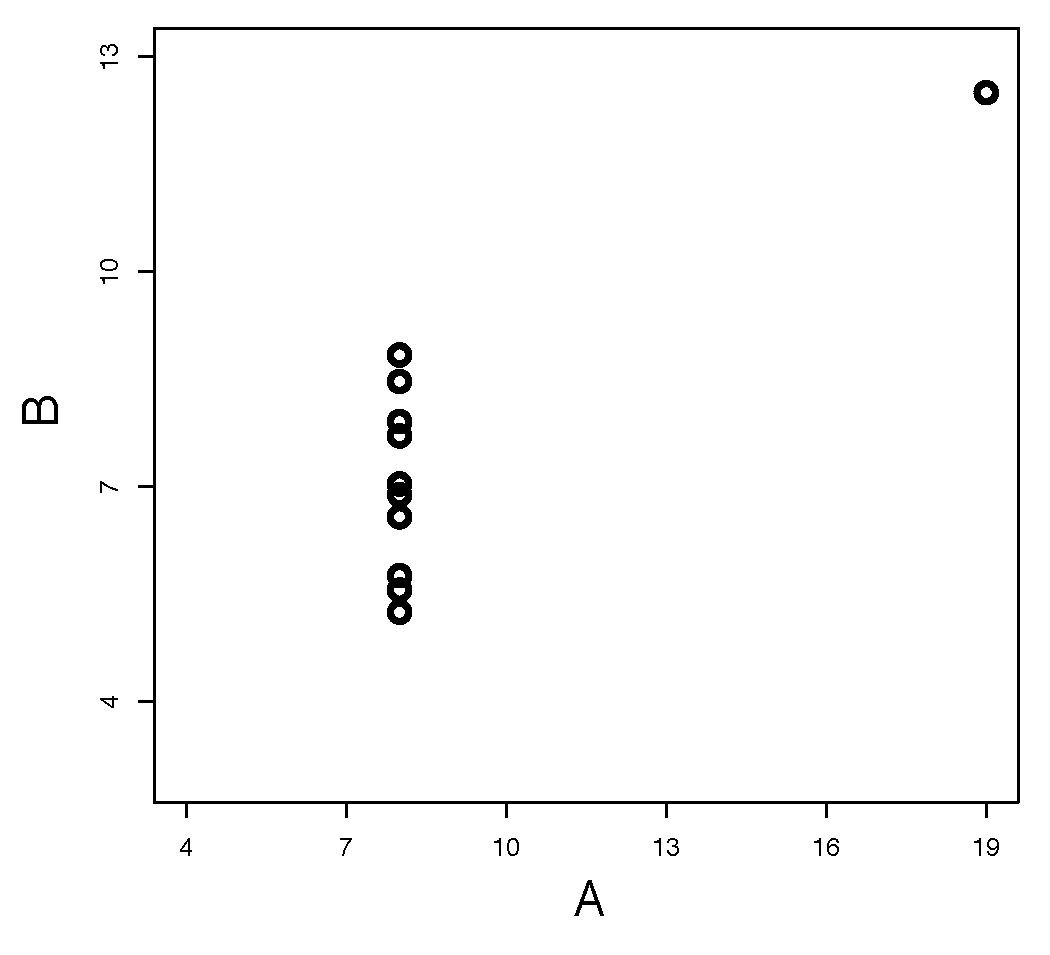
\includegraphics[width=0.4\textwidth]{images/DataEx-Anscombe4.pdf}}
\label{fig:anscombesQuartet}
\end{figure}
\end{frame} 

 \begin{frame} 
\begin{itemize}
\item Perhaps the most important thing to remember in relation to correlation is that \alert{correlation does not necessarily imply causation}.  
\end{itemize}
\end{frame} 

\SectionSlide{Data Preparation}

 \begin{frame} 
\begin{itemize}
\item Some data preparation techniques change the way data is represented just to make it more compatible with certain machine learning algorithms. 
\begin{itemize}
\item Normalization
\item Binning
\item Sampling
\end{itemize}
\end{itemize}
\end{frame} 



\subsection{Normalization}

 \begin{frame} 
\begin{itemize}
\item \keyword{Normalization} techniques can be used to change a continuous feature to fall within a specified range while maintaining the relative differences between the values for the feature. 
\end{itemize}
\end{frame} 

 \begin{frame} 
\begin{itemize}
\item We use \indexkeyword{range normalization} to convert a feature value into the range $\left[low, high\right]$ as follows:
~\\
\begin{equation}
a_i^{'} = \frac{a_i - min(a)}{max(a) - min(a)}\times \left(high-low \right) + low
\label{eq:rangenormalisation}
\end{equation}
\end{itemize}
\end{frame} 

 \begin{frame} 
\begin{itemize}
\item Another way to normalize data is to \keyword{standardize} it into \keyword{standard scores}.
\item A standard score measures how many standard deviations a feature value is from the mean for that feature. 
\item We calculate a standard score as follows:
~\\
\begin{equation}
a_i^{'} = \frac{a_i - \overline{a}}{sd(a)}
\label{eq:standardScore}
\end{equation}
\end{itemize}
\end{frame} 

 \begin{frame} [plain]
The result of normalising a small sample of the \featN{Height} and \featN{Sponsorship Earnings} features from the professional basketball squad dataset.
\begin{table}[htb]
\label{table:normalisationDemo}
\centering
\begin{footnotesize}
\resizebox{\textwidth}{!}{\begin{tabular}{  r | r r r | r r r}
\hline
	&	\multicolumn{3}{c|}{\featN{Height}} &	\multicolumn{3}{c}{\featN{Sponsorship Earnings}}	\\
	&	Values	&	Range	&	Standard	&	Values	&	Range	&	Standard	\\
\hline	

	&	192	&	0.500	&	-0.073	&	561	&	0.315	&	-0.649	\\
	&	197	&	0.679	&	0.533	&	1,312	&	0.776	&	0.762	\\
	&	192	&	0.500	&	-0.073	&	1,359	&	0.804	&	0.850	\\
	&	182	&	0.143	&	-1.283	&	1,678	&	1.000	&	1.449	\\
	&	206	&	1.000	&	1.622	&	314	&	0.164	&	-1.114	\\
	&	192	&	0.500	&	-0.073	&	427	&	0.233	&	-0.901	\\
	&	190	&	0.429	&	-0.315	&	1,179	&	0.694	&	0.512	\\
	&	178	&	0.000	&	-1.767	&	1,078	&	0.632	&	0.322	\\
	&	196	&	0.643	&	0.412	&	47	&	0.000	&	-1.615	\\
	&	201	&	0.821	&	1.017	&	1111	&	0.652	&	0.384	\\
\hline
\textbf{Max}	&	206	&		&		&	1,678	&		&		\\
\textbf{Min}	&	178	&		&		&	47	&		&		\\
\textbf{Mean}	&	193	&		&		&	907	&		&		\\
\textbf{Std Dev}	&	8.26	&		&		&	532.18	&		&		\\
\hline
\end{tabular}}
\end{footnotesize}
\end{table}
\end{frame} 



\subsection{Binning}


\begin{frame} 
\begin{itemize}
\item \keyword{Binning} involves converting a continuous feature into a categorical feature. 
\item To perform binning, we define a series of ranges (called \keyword{bins}) for the continuous feature that correspond to the levels of the new categorical feature we are creating. 
\item We will introduce two of the more popular ways of defining bins: 
\begin{itemize}
\item \keyword{equal-width binning} 
\item \keyword{equal-frequency binning}
\end{itemize}
\end{itemize}
\end{frame} 


 \begin{frame} 
\begin{itemize}
\item Deciding on the number of bins can be difficult. The general trade-off is this:
\begin{itemize}
	\item If we set the number of bins to a very low number we may lose a lot of information 
	\item If we set the number of bins to a very high number then we might have very few instances in each bin or even end up with empty bins.
\end{itemize}
\end{itemize}
\end{frame} 


 \begin{frame} [plain]
\begin{figure}
\begin{tabular}{cc}
\subfigure[3 bins]{\label{fig:binnumber3}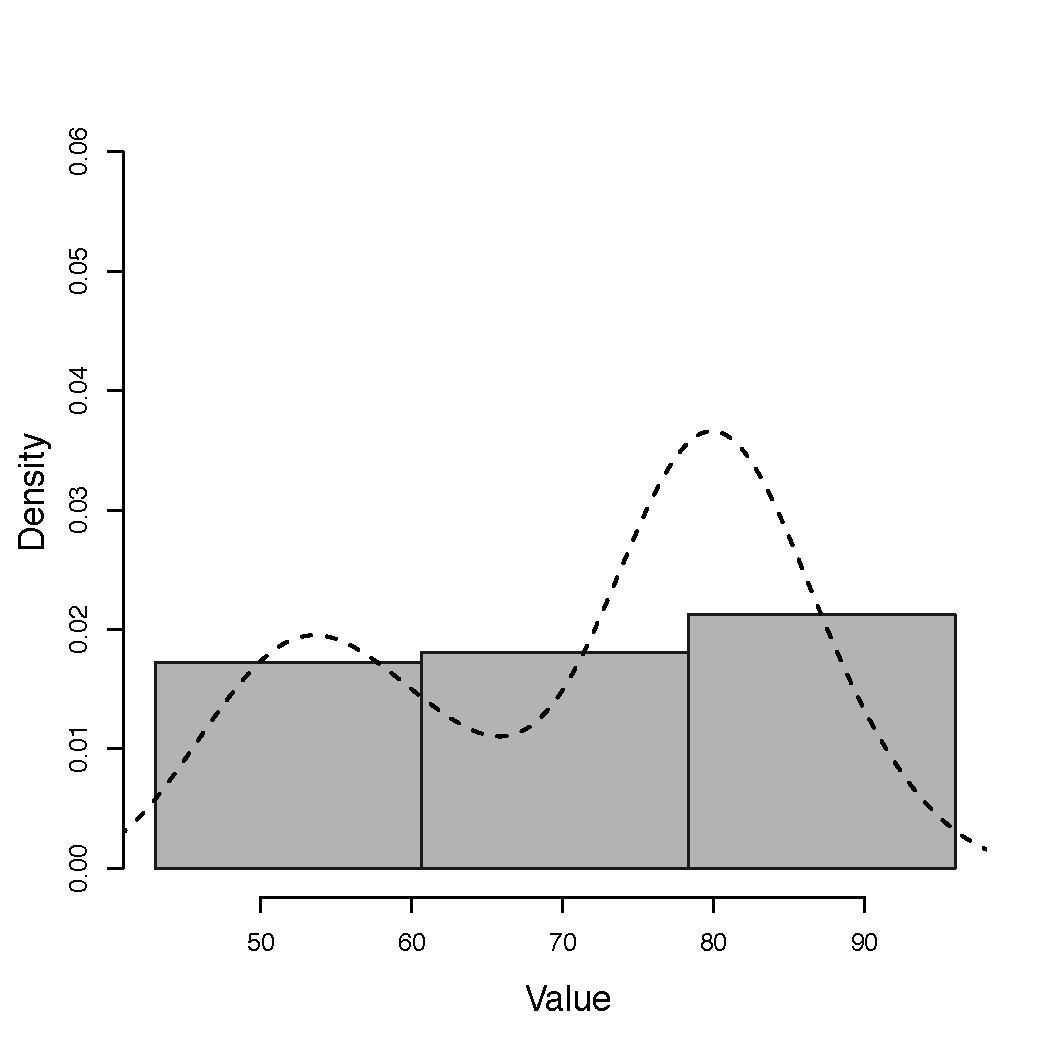
\includegraphics[width=0.36\textwidth]{./images/DifferentBinningDemoHist3.pdf}} &
\subfigure[14 bins]{\label{fig:binnumber14}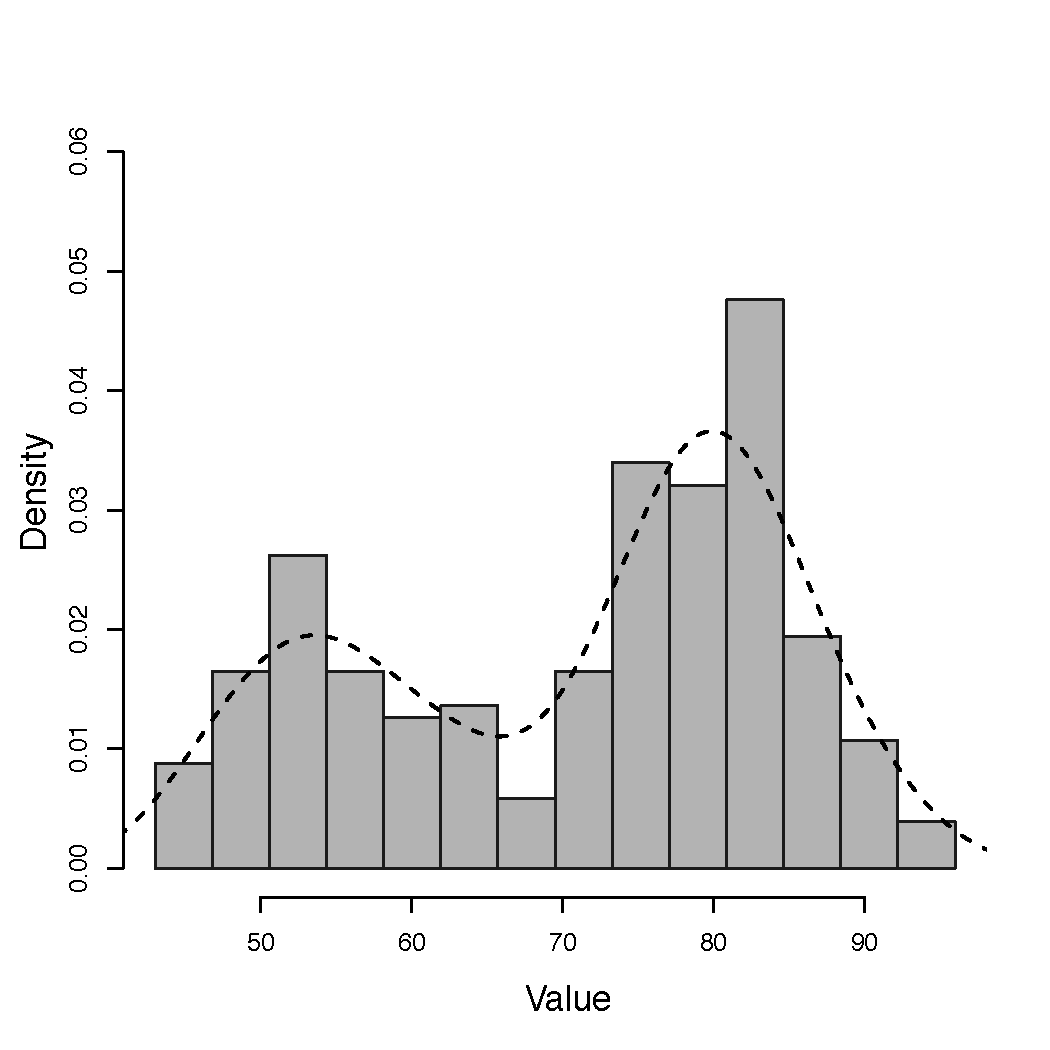
\includegraphics[width=0.36\textwidth]{./images/DifferentBinningDemoHist14.pdf}} \\
\multicolumn{2}{c}{\subfigure[60 bins]{\label{fig:binnumber60}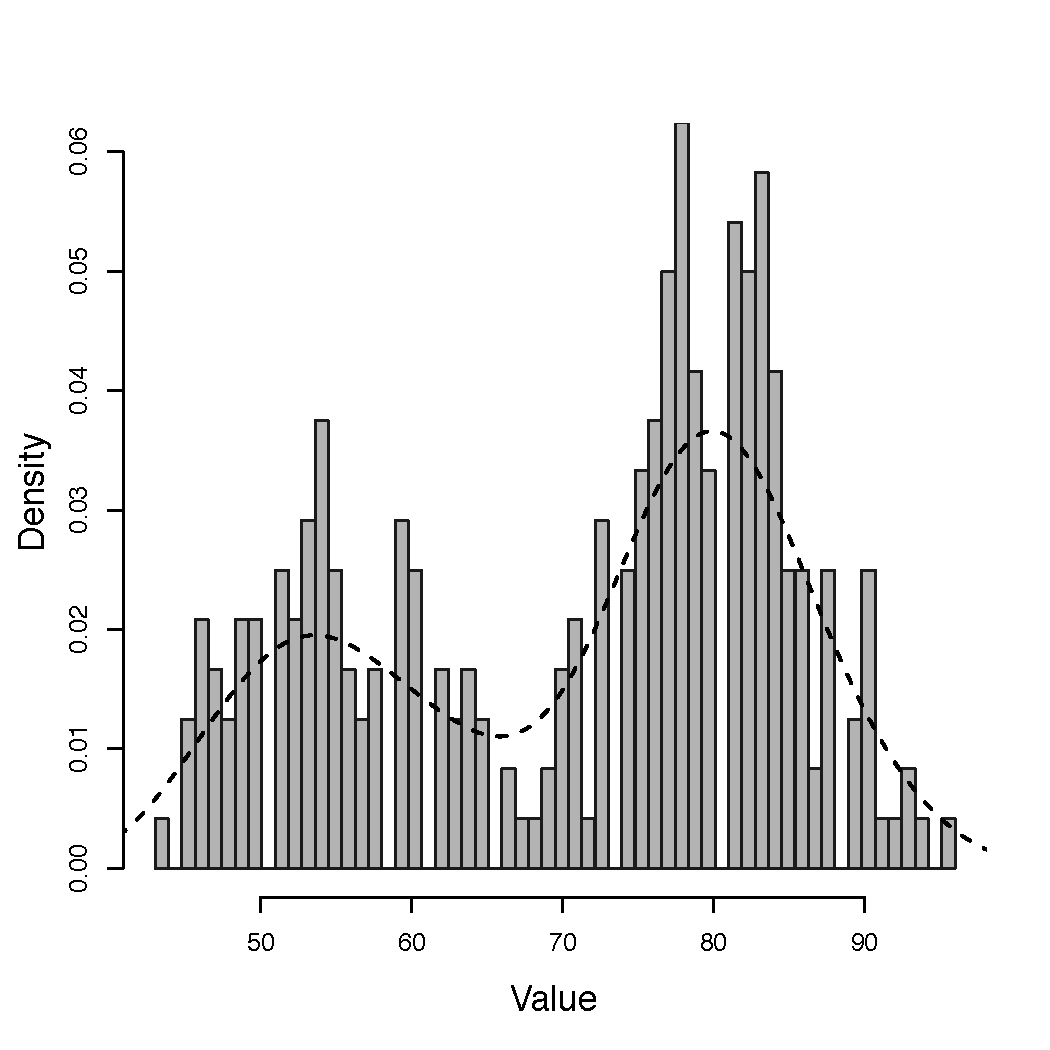
\includegraphics[width=0.36\textwidth]{./images/DifferentBinningDemoHist60.pdf}}} \\
\end{tabular}
\end{figure}
\end{frame} 




 \begin{frame} 
\begin{itemize}
\item The equal-width binning algorithm splits the range of the feature values into $b$ bins each of size $\frac{range}{b}$. 
\end{itemize}
\end{frame} 

 \begin{frame} [plain]
\begin{figure}[!thb]
\centering
\subfigure[5 Equal-width bins]{\label{fig:5equalwidth}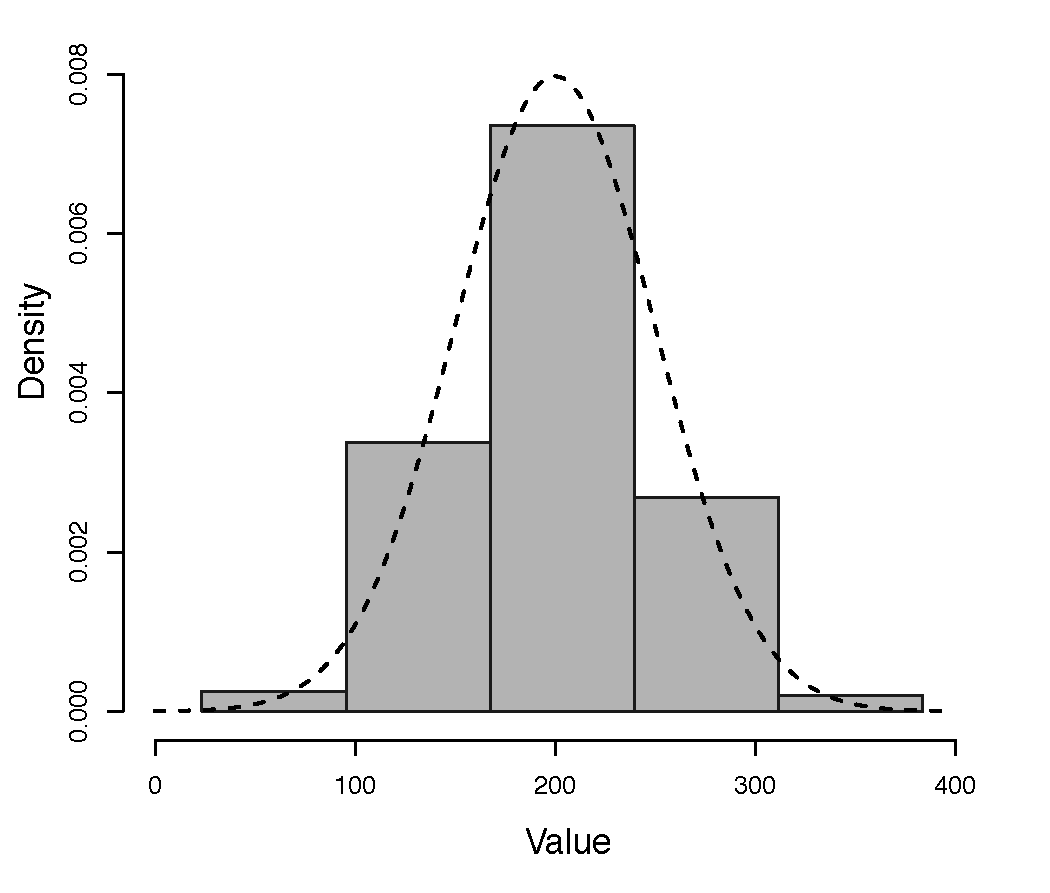
\includegraphics[width=0.35\textwidth]{./images/DifferentBinningStrategyDemoEqualWidth5.pdf}} 
\subfigure[10 Equal-width bins]{\label{fig:10equalwidth}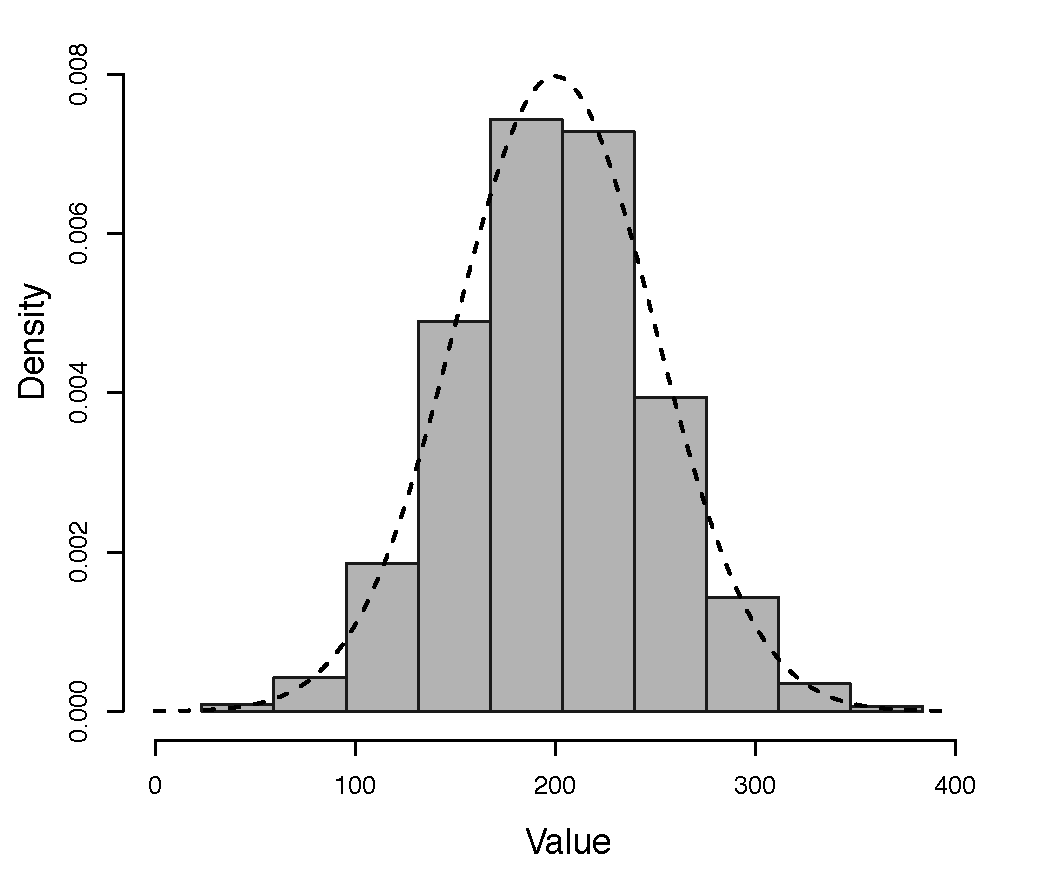
\includegraphics[width=0.35\textwidth]{./images/DifferentBinningStrategyDemoEqualWidth10.pdf}} 
\subfigure[15 Equal-width bins]{\label{fig:15equalwidth}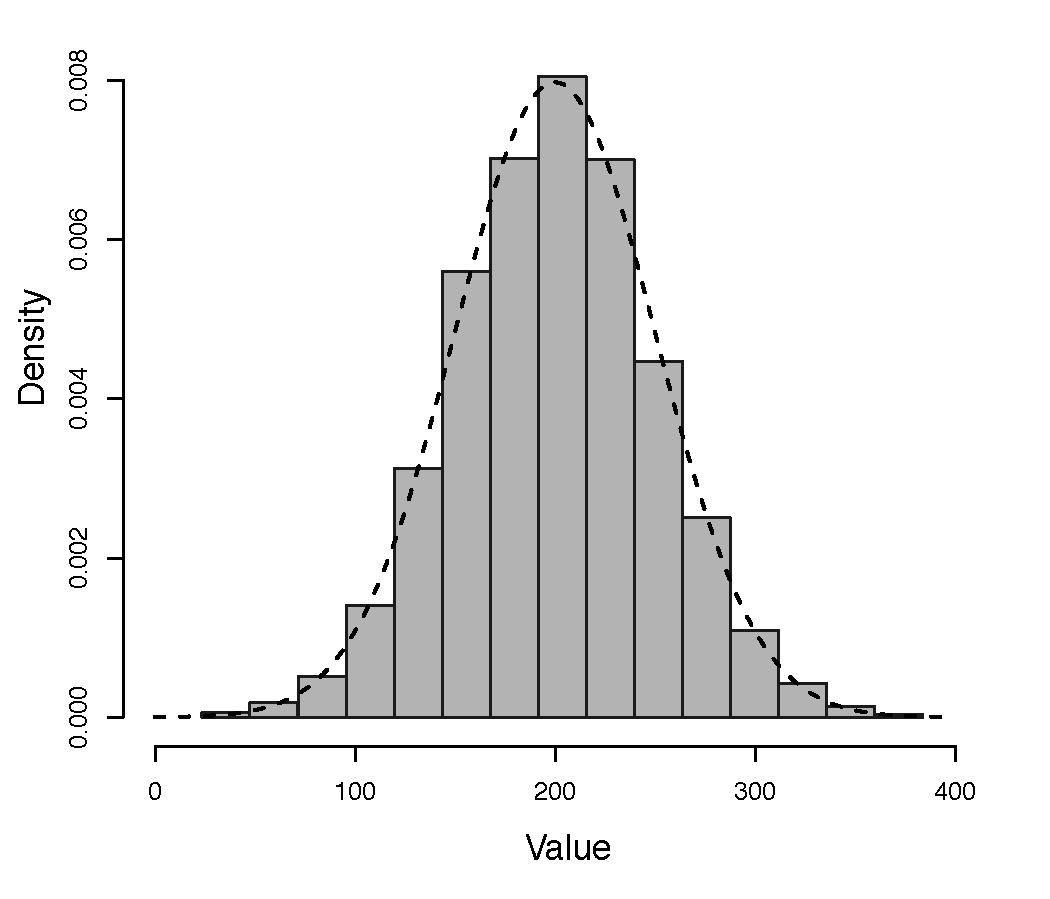
\includegraphics[width=0.35\textwidth]{./images/DifferentBinningStrategyDemoEqualWidth15.pdf}} 
\end{figure}
\end{frame} 

 \begin{frame} 
\begin{itemize}
\item \keyword{Equal-frequency binning} first sorts the continuous feature values into ascending order and then places an equal number of instances into each bin, starting with bin 1. 
\item The number of instances placed in each bin is simply the total number of instances divided by the number of bins, $b$. 
\end{itemize}
\end{frame} 

 \begin{frame} [plain]
\begin{figure}[!thb]
\centering
\subfigure[5 Equal-frequency bins]{\label{fig:5equalfrequency}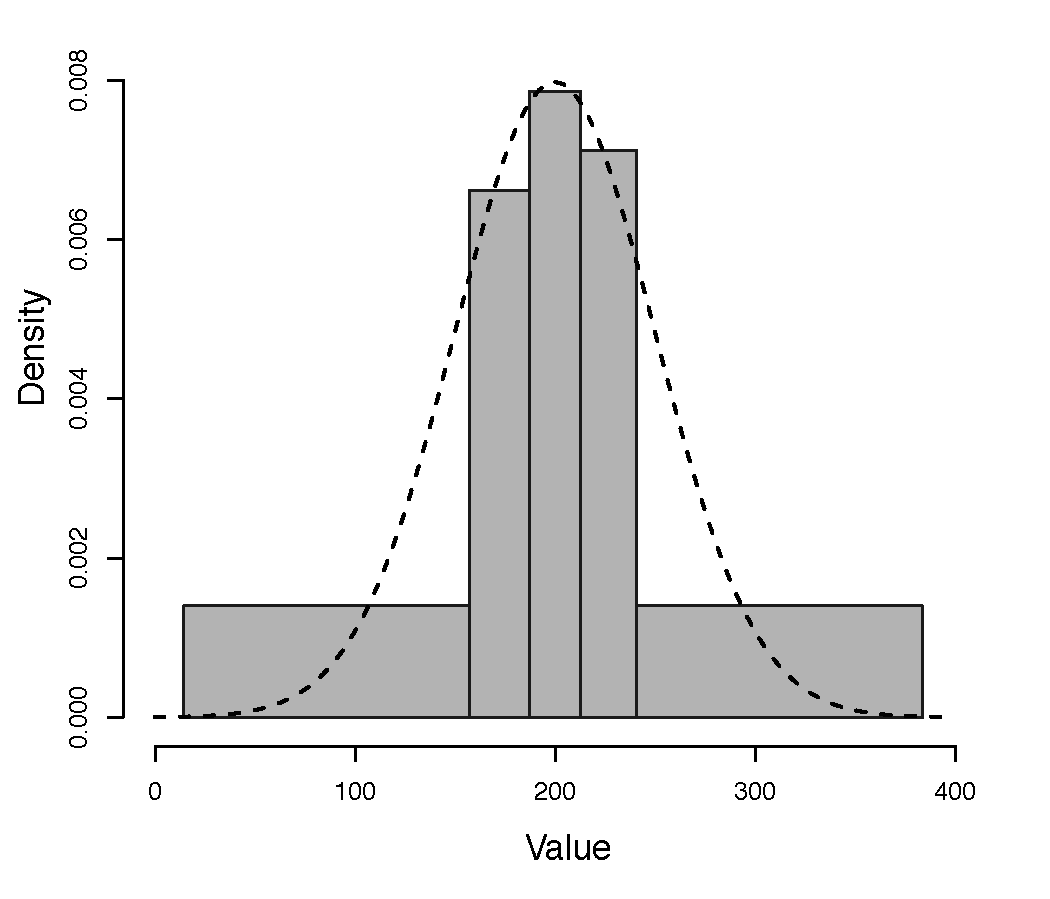
\includegraphics[width=0.35\textwidth]{./images/DifferentBinningStrategyDemoEqualFrequency5.pdf}} 
\subfigure[10 Equal-frequency bins]{\label{fig:10equalfrequency}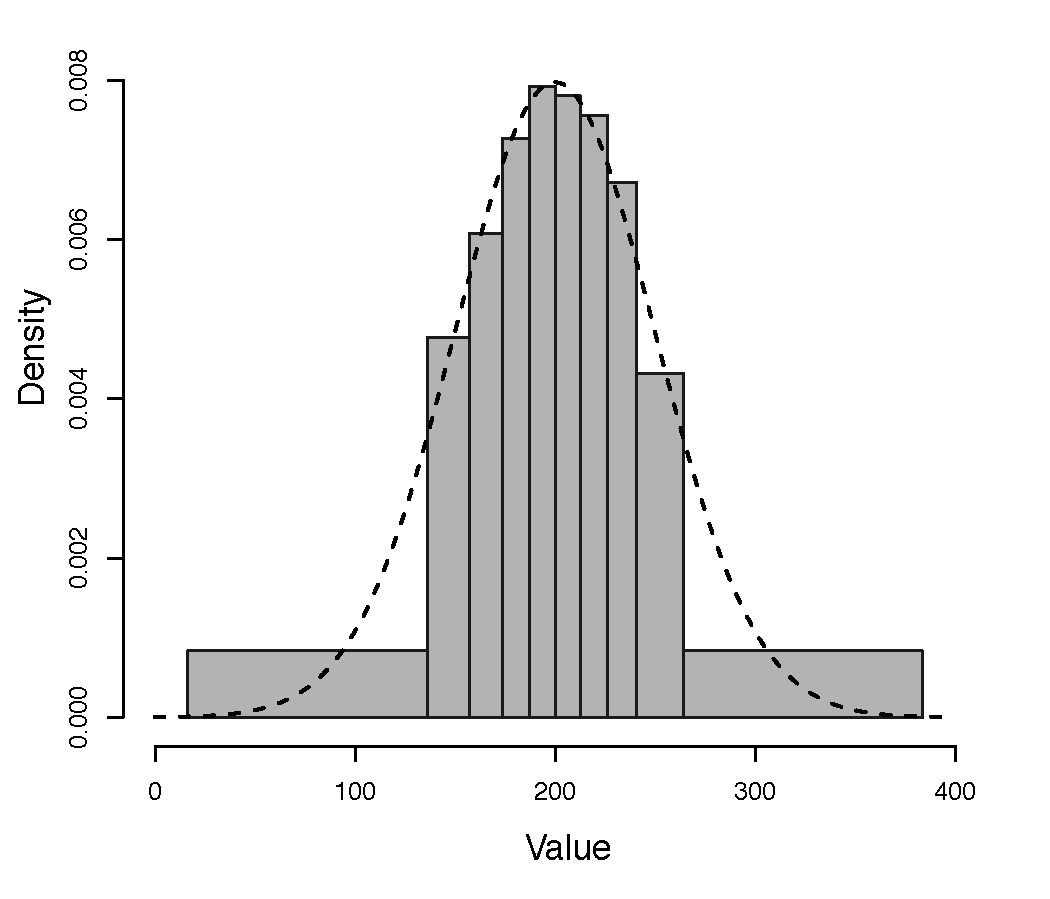
\includegraphics[width=0.35\textwidth]{./images/DifferentBinningStrategyDemoEqualFrequency10.pdf}}
\subfigure[15 Equal-frequency bins]{\label{fig:15equalfrequency}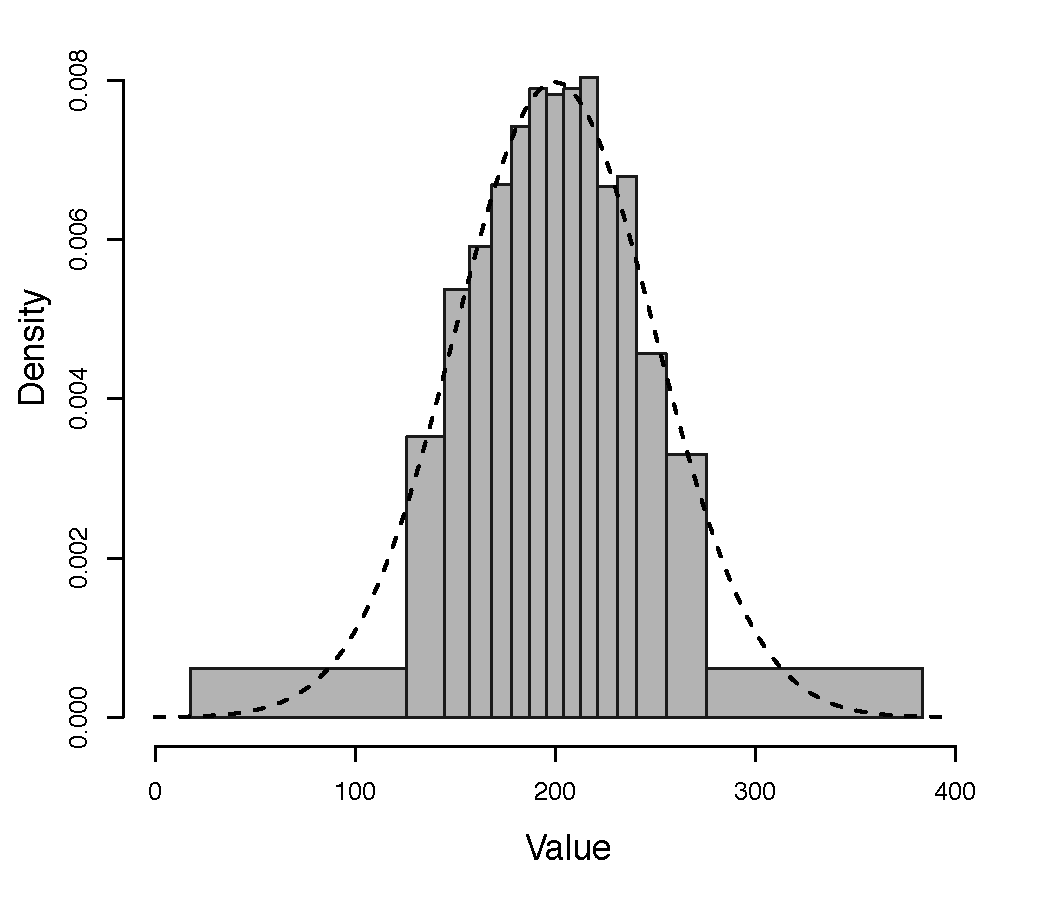
\includegraphics[width=0.37\textwidth]{./images/DifferentBinningStrategyDemoEqualFrequency15.pdf}}
\end{figure}
\end{frame} 

\subsection{Sampling}


 \begin{frame} 
\begin{itemize}
\item Sometimes the dataset we have is so large that we do not use all the data available to us in an ABT and instead \keyword{sample} a smaller percentage from the larger dataset. 
\item We need to be careful when sampling, however, to ensure that the resulting datasets are still representative of the original data and that no unintended \keyword{bias} is introduced during this process. 
\item Common forms of sampling include:
\begin{itemize}
\item \keyword{top sampling}
\item \keyword{random sampling}
\item \keyword{stratified sampling}
\item \keyword{under-sampling}
\item \keyword{over-sampling}
\end{itemize}
\end{itemize}
\end{frame} 


 \begin{frame} 
\begin{itemize}
\item \keyword{Top sampling} simply selects the top $s\%$ of instances from a dataset to create a sample. 
\item Top sampling runs a serious risk of introducing bias, however, as the sample will be affected by any ordering of the original dataset. 
\item We recommend that top sampling be avoided.
\end{itemize}
\end{frame} 

 \begin{frame} 
\begin{itemize}
\item Our recommended default, \keyword{random sampling} randomly selects a proportion of $s\%$ of the instances from a large dataset to create a smaller set. 
\item Random sampling is a good choice in most cases as the random nature of the selection of instances should avoid introducing bias.
\end{itemize}
\end{frame} 

 \begin{frame} 
\begin{itemize}
\item \keyword{Stratified sampling} is a sampling method that ensures that the relative frequencies of the levels of a specific \keyword{stratification feature} are maintained in the sampled dataset. 
\item To perform stratified sampling:
\begin{itemize}
\item the instances in a dataset are  divided into groups (or strata), where each group contains only instances that have a particular level for the stratification feature
\item  $s\%$ of the instances in each stratum are randomly selected
\item these selections are combined to give an overall sample of $s\%$ of the original dataset. 
\end{itemize}
\end{itemize}
\end{frame} 



 \begin{frame} 
\begin{itemize}
\item In contrast to stratified sampling, sometimes we would like a sample to contain different relative frequencies of the levels of a particular feature to the distribution in the original dataset. 
\item To do this, we can use \keyword{under-sampling} or \keyword{over-sampling}. 
\end{itemize}
\end{frame} 

 \begin{frame} 
\begin{itemize}
\item \keyword{Under-sampling} begins by dividing a dataset into groups, where each group contains only instances that have a particular level for the feature to be under-sampled. 
\item The number of instances in the \textit{smallest} group is the under-sampling target size. 
\item Each group containing more instances than the smallest one is then randomly sampled by the appropriate percentage to create a subset that is the under-sampling target size. 
\item These under-sampled groups are then combined to create the overall under-sampled dataset.
\end{itemize}
\end{frame} 

 \begin{frame} 
\begin{itemize}
\item \keyword{Over-sampling} addresses the same issue as under-sampling but in the opposite way around. 
\item After dividing the dataset into groups, the number of instances in the \textit{largest} group becomes the over-sampling target size. 
\item From each smaller group, we then create a sample containing that number of instances using \keyword{random sampling with replacement}. 
\item These larger samples are combined to form the overall over-sampled dataset. 
\end{itemize}
\end{frame} 

\SectionSlide{Summary}

\begin{frame} 
\begin{itemize}
\item The key outcomes of the \keyword{data exploration} process are that the practitioner should
\begin{enumerate}
\item Have \emph{gotten to know} the features within the ABT, especially their central tendencies, variations, and \keyword{distributions}{probability distribution}.
\item Have identified any \keyword{data quality issues} within the ABT, in particular \keyword{missing values}, \keyword{irregular cardinality}, and \keyword{outliers}.
\item Have corrected any data quality issues due to \keyword{invalid data}.
\item Have recorded any data quality issues due to \keyword{valid data} in a \keyword{data quality plan} along with potential handling strategies.
\item Be confident that enough good quality data exists to continue with a project.
\end{enumerate}  
\end{itemize}
\end{frame} 

\begin{frame}
	\tableofcontents
\end{frame}



\end{document}
